\documentclass[11pt,a4paper]{article}

\usepackage [spanish]{babel}
\usepackage [utf8]{inputenc}
%\usepackage[latin1]{inputenc}para utilizar acentos pero aqui no funciona (en otros si)
\usepackage [T1]{fontenc}
\usepackage{graphicx}
\usepackage{graphics}
\graphicspath{ {Figuras/} } %Para buscar las imágenes en otra carpeta
\usepackage{amsfonts} %Para poder escribir letras como la matriz identidad
\usepackage{mathrsfs} %Para poder escribir letras como la H del el espacio de Hilbert
\usepackage{slashed} % para la d barra cruzada
\usepackage{amsmath}
\usepackage{amssymb}
\usepackage{makeidx}
\usepackage{hepunits} %para poder utilizar unidades
\usepackage[version=3]{mhchem} %para poder escribir los simpolos atómicos y químicos
%\usepackage{hep}
\usepackage[left=2.5cm,right=2.5cm,top=2.5cm,bottom=2.5cm]{geometry}
\usepackage [labelformat=empty]{caption}
%\usepackage{wrapfig} %for I can use wrapfigure
\usepackage[font={small, up}]{caption}
\usepackage[caption = false]{subfig}
\usepackage{hyperref} %hipervinculos del índice
\setlength{\parindent}{4em} %para que interprete la linea en blanco como un \parragraph{}
\setlength{\parskip}{1em}
%\setbeamertemplate{caption}[numbered]%numerar imágenes


\renewcommand{\baselinestretch}{1.15}
\renewcommand{\thefigure}{}

%para aumentar el espacio entre elementos del índice
\usepackage{setspace}

\bibliographystyle{unsrthep}



\begin{document}

\begin{titlepage}

\begin{center}
\vspace*{-1in}
\vspace*{1 cm}
\begin{figure}[htb]
\begin{center}

\includegraphics[scale=1]{Logo1.png}
\end{center}
\end{figure}
\vspace*{2 cm}


{\large MÁSTER EN FÍSICA AVANZADA}\\
\vspace*{0.2in}
{\huge Especialidad en física nuclear y de partículas}\\
\vspace*{0.2in}
\vspace*{0.6in}
\end{center}
\vspace*{-1in}
\begin{center}

\begin{figure}[htb]
\begin{center}

\includegraphics[scale=0.1]{Logo2.jpg} 
\end{center}
\end{figure}
\vspace*{1 cm}

\begin{large}
\textbf{{\large Trabajo final de máster}}\\
\rule{80mm}{0.1mm}\\
%\vspace*{2 cm}

\end{large}
\vspace*{0.2in}
\begin{Large}
\textbf{Diseño de un detector de aguas tritiadas basado en fibras centelleadoras leidas por fotomultiplicadores de silicio} \\
\end{Large}
%\vspace*{0.3in}
\vspace*{2 cm}

\begin{large}
Marcos Martínez Roig\\
\end{large}
\end{center}

\vspace*{0.3in}
%\rule{80mm}{0.1mm}\\
\vspace*{0.1in}
\begin{large}
\begin{flushright}
\item[\bf Tutores:\hspace{4cm} ]\quad  \\ José Díaz Medina\\
Nadia Yahlali Haddou\\
\end{flushright}
\end{large}

\end{titlepage}

%\input{./Secciones/abstract}

%\newpage
\tableofcontents
\newpage

%%%%%%%%%%%%%%%%%%%%%%%%%%%%%%% MAIN BODY %%%%%%%%%%%%%%%

\section{Introduccion}  \label{sec:ch01}
Hoy en día existe un problema que concierne  las  centrales nucleares de fisión, central termoeléctrica,  experimento de física de partículas, etc., e, incluso, en futuras centrales de fusión nuclear y es la creación de altos niveles de radiactividad en estos sitios. Por ejemplo, una central nuclear operando en modo normal puede llegar a emitir alrededor de $300\ \tera\becquerel/\giga\watt\mathrm{y}$ ~\cite{300TBq}.  Debido a la peligrosidad que ello implica estos deben ser controlados y disminuidos en la medida de lo posible.

En concreto, uno de los elementos radiactivos más abundantes generados en estos lugares es el tritio. Debido a las elevadas tasas de radiactividad anteriormente mencionada,es fundamental controlarlo en estas zonas de trabajo para evitar que contribuya a esta cifra ya que un mayor número de emisiónes radiactivas se traduce en una mayor posibilidad de que ello afecte a diversos elementos, entre ellos la salud de las personas.

Para que podamos entender la facilidad con la que este se produce el tritio hay que tener en cuenta que este es el tercer isótopo de hidrógeno formado por un protón y dos neutrones. Por un lado, el hidrógeno es uno de los elementos más abundantes de la tierra y, por otro lado, en cualquier lugar de los anteriormente mencionados, se necesita elevar la temperatura para conseguir que, las reacciones en las que se basa su funcionamiento, puedan ocurrir (para abrir el canal de dicha reacción o aumentar la probabilidad de producirse). Como resultado de ello se producen con bastante asiduidad neutrones con energía suficiente para considerase cuasilibres. 

Podemos entender entonces que, en estos lugares y en estas condiciones, dada la alta tasa de hidrógeno y neutrones, existe una posibilidad relativamente alta de que aparezca tritio o de que existan diversos elementos que puedan dar lugar a la creación de tritio. Algunos de los principales canales de creación de tritio son la captura neutronica del $\ce{^6Li}$, $\ce{^7Li}$, $\ce{H}$, etc. las cuales se muestran a continuación:
\begin{equation}
\ce{^{6}Li} + n \rightarrow \ce{T} + \ce{^{4}He}
\label{capneuLi6}
\end{equation}
\begin{equation}
\ce{^{7}Li} + n \rightarrow  \ce{T} + \ce{^{4}He} + n
\label{capneuLi7}
\end{equation}
\begin{equation}
\ce{^{1}H} + 2n \rightarrow  \ce{T}  
\label{capneuH}
\end{equation}
%$\eqref{capneuLi6}$ para referenciar ecuaciones

Según nuestro planteamiento también será más facil todavía que se produzca deuterio, segundo isótopo del hidrógeno (compuesto por un protón y un neutrón). Esto es verdad pero ello no nos importa para nuestro objetivo debido a que el deuterio no es un isótopo radiactivo.

Como hemos dicho, el tritio es el tercer isótopo del hidrógeno compuesto por un proton y dos neutrones (referencia). Se trata de un elemento radiactivo con un periodo de semidesintegración de $12.32$ años, en concreto, un emisor $\beta^-$ de baja energía que emite electrones según la siguiente reacción:
\begin{equation}
T \rightarrow \ce{^{3}He} + e^- + \overline{\nu}_e
\label{desintegraciontritio}
\end{equation}
Donde lo que ha ocurrido es que uno de los neutrones que conforman el tritio se ha desintegrado (a partir de una interacción débil) de acuerdo a una desintegración $\beta^-$ en un protón, un electrón y un antineutrino electrónico:
\begin{equation}
n \rightarrow p + e^- + \overline{\nu}_e \qquad \rightarrow \qquad (pnn)_T\rightarrow (ppn)_{^3He} + e^- + \overline{\nu}_e 
\label{desintegracionbeta}
\end{equation}
La existencia de este antineutrino electrónico es impuesta por la conservación del numero leptónico, en concreto el número leptónico de la familia del electrón ($L_e$). En la práctica no tenemos la posibilidad de detectar esta partícula ya que interacciona muy débilmente con la materia ($\sigma \propto 10^{-42}~\cm^2$) y por tanto con el material que conforma nuestro detector (en concreto fibras centelleadores BCF-12). Es decir, esta partícula escapa sin interaccionar con el detector y en su lugar solo detectamos su ausencia, es decir, la no conservación de ciertas cantidades físicas como energía, momento, número leptónicos, etc. en la totalidad de las partículas detectadas.

Por tanto solo tenemos la posibilidad de detectar el isotopo $\ce{^3He}$ , isótopo estable, y el electrón. Hay que tener en cuenta que, aunque el isótopo hijo de la reacción de desintegración del tritio, $\ce{^3He}$ , sea estable (presenta una vida media infinita, es decir, no se desintegra) realmente este se encontrará en un estado no estacionario, es decir, no se encuentra en un autoestado de su hamiltoniano, sino en un estado que puede expresarse como una la suma de autoestados del hamiltoniano. Como consecuencia, tras la desintegración $\beta^-$ del tritio tendremos una posterior desexcitación del $\ce{^3He}$ que producirá fotones con varias energías bien definidas que corresponden a sus niveles energéticos, fotones que podremos observar en nuestro detector. En resumen obtendremos un espectro de desintegración del tritio junto a un espectro típico de rayos X, espectro idealmente discreto pero experimentalmente gaussiano debido a diversas incertidumbres tales como la de los aparatos de medida.

Dado que el $\ce{^3He}$  presenta una masa muy superior a la de los electrones, por conservación de energía y momento podemos observar que el $\ce{^3He}$  apenas se moverá del sitio donde ha ocurrido la reacción. Por tanto nos centraremos en la detección del electrón. En la figura uno podemos apreciar el espectro energético de los electrones emitidos en la desintegración del tritio.

\begin{figure}[hbtp]
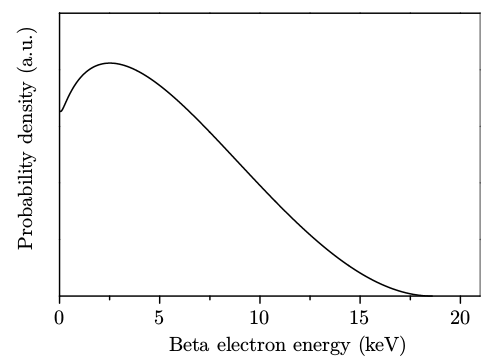
\includegraphics[scale=0.6]{Espectro.png}
\centering
\caption{Espectro energético de los electrones de la desintegración del tritio ~\cite{TesisTritio}}
\end{figure}

Como era de esperar, este presenta la forma típica de un espectro energético de una desintegración $\beta$. Podemos observar que estos poseen una energía máxima de $18.6~\keV$, una energía promedio de $5.7~\keV$ y una moda (valor más probable) lígeramente inferior a la energía promedio, entorno a $4.5~\keV$. Con estos valores de energía podemos apreciar que la energía de radiación del tritio es la más pequeña observada hasta el momento en los isótopos. Como consecuencia el electrón presentará un recorrido libre medio muy corto, del orden de $3-5~\mm$ en el aire y de $5-6~\mu m$ en la fibra centelleadora.

El problema actual reside en que los mecanismos de detección y monitorización de tritio utilizados en la actualidad, en concreto en centrales nucleares, que será el objetivo final del detector que pretendemos desarrollar en el grupo experimental internacional denominado \textit{Tritium}, son métodos lentos o con un alto umbral de detección ~\cite{limiteMB}~\cite{Limitetiempo}~\cite{Limite}. 

Por ejemplo, entre los métodos más empleado actualmente en centrales nucleares, esta el método de detección de aguas tritiadas por medio de centelleo líquido. Este es el método más indicado para la detección de partículas beta de energía muy pequeña porque, como ya se ha visto al analizar el espectro energético de los electrones que conforman la radiación $\beta$ del tritio estos presentan un recorrido libre medio muy pequeño (del orden del mm o $\mu m$, dependiendo del medio (referencia)). Dado que solo contribuye a la medida (con una probabilidad aceptable) las emisiones que han tenido lugar a una distancia del detector inferior al recorrido libre medio la forma más efectiva de conseguir que un mayor volumen de la fuente radiactiva contribuya a la señal y que un mayor volumen del detector se encuentre a una distancia adecuada de la fuente radiactiva es disolviendo este detector con el líquido radiactivo (en nuestro caso agua tritiada), y esto solo se puede conseguir utilizando detectores líquidos de partículas beta, como el liquido centelleador. 

El método de centelleo líquido consiste en tomar una muestra del líquido radiactivo, agua tritiada en nuestro caso, diluirla (habitualmente al 50\%) con el líquido centelleador y medir los fotones emitidos por este líquido centelleador, a partir de los cuales podremos determinar los electrones emitidos por la muestra de agua tritiada y detectados por el líquido centelleador. Sin embargo para ello se necesita tomar una muestra y llevarla al laboratorio para el correspondiente estudio. En resumen se trata de un proceso de detección de agua tritiada basado en metodos offline que ralentizan la monitorización dilatando el resultado hasta varios dias desde la toma de la muestra. 

Tras cada análisis, la muestra de agua tritiada y líquido centelleador son inseparable y por tanto no reutilizable.  Este debe de ser tratado como residuo peligroso ya que, aunque el análisis desvele que el agua tritiada esta libre de tritio (presente una actividad suficientemente baja para ser tratada como material no radiactivo), esta contiene tolueno, presente en el líquido centelleador y, por tanto, debe de ser procesada de manera segura. También necesita operarios especializados manipulen estas muestras, poniendo en peligro su salud ~\cite{gel}.

El objetivo final de \textit{Tritium}, sobre el cual tratará mi futura tésis, es desarrollar un detector de aguas tritiadas que permita realizar la monitorización del tritio \textit{in situ} a tiempo real. Por tiempo real entendemos una dilatación temporal máxima de 10 minutos desde la toma de la muestra (ya que se necesita un tiempo mínimo para poder discernir la señal del background, el cual dependera, entre otras cosas, de la configuración del sistema de detección). Además el prototipo desarrollado no necesitará de la presencia de personal especializado que intervenga en el proceso de monitorización de aguas tritiadas, agilizando y abaratando el método de monitorización, además de excluir posibles errores humanos. El método simplemente requerirá continuas calibraciones al cabo de un tiempo determinado para asegurar el correcto funcionamiento del dispositivo. 

La dificultad aquí residirá en conseguir extraer esta señal tan pequeña ($\backsim 1~\keV$) y tener estadística suficiente para poder discernirla del fondo radiactivo en un tiempo tan pequeño. El proyecto \textit{Tritium} pretende llegar a realizar detecciones en el límite de actividades de la muestra de agua tritiada entorno a $0.1$ o $1~\kilo\becquerel/L$ lo cual nos permitirá dar mesajes de alarma cuando la muestra supere el límite recomendado por la Comunidad Europea, $100\becquerel/L$. Los trabajos \textit{in situ} con configuraciones del detector similares (centelleador + contador de fotones) realizados hasta la fecha que utilizan el concepto de tiempo real solo han conseguido obtener una señal en el límite del MeV/L ~\cite{TesisTritio} o incluso decenas de kBq/L~\cite{Rat}. Estos estan basados principalmente en solidos centelleadores y tubos fotomultiplicadores (PMT) a diferencia de nuestro experimento que consta de fibras centelleadoras (que detectan la radiación beta del tritio y la convierten en fotones) y tubos fotomultiplicadores o fotomultiplicadores de silicio (que detectan estos fotones y los convierten en electrones que conformarán la señal del sistema). 

En mi opinion el uso de fibras centelleadores es una mejor elección ya que presentan un mayor volumen activo con el que detectar el la radiación del tritio  sin necesidad de utilizar líquido centelleador el cual, como he mencionado anteriormente, produce residuos peligrosos además del coste del líquido centelleador no reutilizable. Además las fibras centelleadoras presentan un mayor abanico de posibilidades en cuanto a la elección de las distintas estructuras de las mismas. Nuestro experimento se centrará en la utilización de SiPM aunque también contemplará el uso de PMT. 

Hay que tener en cuenta que si existen diseños que logran llegar a límites del orden del Bequerelio en un tiempo de 3 minutos, aunque estos estan basados en configuraciones totalmente distintas, como por ejemplo un sistema, conformado por un láser y cavidades espectroscópicas en forma de anillo, en el cual se pretende buscar la existencia de resonacias y relacionar las frecuencias a las que estas ocurren con la concentración de tritio presente en la muestra. ~\cite{Anillo}. Sin embargo este es un estudio totalmente diferente ya que necesita de un acondicionamiento y control exhaustivo de las condiciones del sistema para el correcto funcionamiento del láser, encareciendo la construcción y mantenimiento del mismo y dificultando la existencia de este en sitios como centrales nucleares, es decir, es una aplicación que no persigue un mismo fín. 

Para conseguir extraer una señal tan pequeña con la mayor eficiencia posible estudiaremos diversas configuraciones experimentales para conseguir obtener la mas adecuada de acuerdo a nuestro objetivo experimental. Además realizaremos en todo momento detecciones en coincidencia, lo cual nos permitira eliminar en gran medida el fondo radiactivo del experimento. Las configuraciónes que pretendemos abarcar en el experimento son: 
\begin{itemize}
\item {}
Por un lado estudiaremos cual es la mejor elección para las estructuras de fibras centelleadores. Estudiaremos las ventajas y desventajas que presenta la utilización clads en las fibras (recubrimiento de la fibra centelleadora para evitar la fuga de fotones de centelleo y poder dirigir estos de manera opticamente aceptable hasta el contador de fotones). 
\item {}
Por otro lado estudiaremos cual es la mejor elección para un contador de fotones. Las posibilidades contempladas en el experimento serán SiPM o PMT. Veremos cual es más adecuado ya que cada una presenta una serie de características mejores como la eficiencia de fotodetección (PDE) de los SiPM sobre la de los PMT pero otras tantas peores como la dependencia con la temperatura más acusada en los SiPM que en los PMT.
\end{itemize}

También se realizarán una serie de simulaciones del experimento previas al desarrollo del mismo utilizando el programa "Geant 4", desarrollado por el cern, con el objetivo de ver que es el que deberíamos esperar teóricamente de nuestros resultados. Estas simulaciones nos permitiran comparar nuestros resultados experimentales con los datos simulados para ver hasta que punto nuestro experimento dista del modelo teórico seguido, lo cual nos permitira a su vez comprobar la fiabilidad de este modelo teórico y corregir posibles erratas del mismo. También nos permitirá ver que posibles modificaciones podemos realizar en el experimento para obtener un mejor resultado.

El grupo experimental \textit{Tritium} es un grupo internacional compuesto por tres paises: Portugal, Francia y España; En concreto intervienen las universidades de...  El proyecto que planteamos en este grupo es demasiado extenso para una trabajo de fín de master ya que se necesitan años para conseguir resultados concluyentes y, como ya se ha mencionado anteriormente, será la base de mi futura tésis. En este trabajo de fin de máser únicamente nos centraremos en los primeros pasos de este gran proyecto, el cual ha empezado recientemente y, afortunadamente, me ha permitido estar en este desde el inicio.

Dividiremos este trabajo en seis partes:
\begin{enumerate}
\item{} En primer lugar se realizará un pequeño estudio sobre las fibras centelleadoras. Por un lado se determinará cual es la forma adecuada de actuar a la hora de manipular fibras centelleadoras, elemento más sensible de los utilizados en el experimento, presentando el procedimiento final de como preparar un bunch de fibras centelleadoras con resultado opticamente aceptable. Por otro lado se utilizarán distintas estructuras de las mismas para ver cual nos permite obtener una señal del agua tritiada  más óptima. 

\item{} En segundo lugar realizaremos una calibración de los SiPM, paso fundamental antes de poder obtener cualquier medida del experimento. La finalidad de este paso es poder catalogar la magnitud de la medida del sistema que estamos obteniendo con este instrumento, algo fundamental en física. No se necesita realizar una calibración de los PMT, paso igualmente importante al anterior, ya que este trabajo fue realizado recientemente por otro componente del grupo.

\item{} En tercer lugar se describirá uno de las posibles configuraciones que serán estudiadas con el fin de determinar cual de estas es la más adecuada, desde el punto de vista del objetivo final de proyecto, para el diseño final del detector. Este también nos permitirá encontrar posibles fallos y mejoras que optimicen nuestro prototipo y que podrán ser utilizadas para el diseño final. En concreto la configuración que se estudiará esta formada por un bunch de 35 fibras centelleadoras sin clad leidas por PMT. También se hablará, entre otras cosas, del proceso de llenado que tuvo que ser desarrollado para una realización segura del mismo además del los resultados obtenidos.

\item{} En cuarto lugar se presentarán las simulaciones realizadas con el programa de Geant4, programa desarrollado por el cern capaz de realizar simulaciones muy detalladas de experimentos, principalmente de física de partículas. En este punto se presentaran las simulaciones realizadas tanto para los prototipos como para posibles diseños finales. Esto nos permitirá ver que posibles mejoras podemos incluir a nuestro experimento y en que puntos difieren los resultados obtenidos con las simulaciones con los resultados obtenidos en los distintos experimentos de los prototipo.

\item{} En quinto lugar se presentará se comentaran posibles partes del experimento que queden inconclusas o inacabadas o puntos interesantes y que serán propuestos a futuros estudios que habrá que realizar durante la tésis. También se comentará brevemente el siguiente paso que pretenderemos realizar en el proyecto.

\item{} Se presentará un último punto donde se expondrán las conclusiones alcanzadas durante la completitud del trabajo.

\end{enumerate}

\newpage
\section{Protocolo de manipulación de fibras centelleadoras} \label{sec:ch03}
Como se ha comentado anteriormente, el primer paso para monitorizar el agua tritiada es detectar los electrones que se producen en la desintegración $\beta^-$ del tritio $\eqref{desintegraciontritio}$. Para ello se utilizarán fibras centelleadoras cuya oferta ofertada existente en el mercado se estudió~\cite{Alberto} y se determino que las fibras BCF-12 eran las que mejor se ajustaban a los requisitos del experimento. 

Un elemento centelleador esta formado por materiales luminiscentes cuyos átomos o moléculas que los componen presentan unos niveles energéticos similares a los de la figura dos:

\begin{figure}[hbtp]
\centering
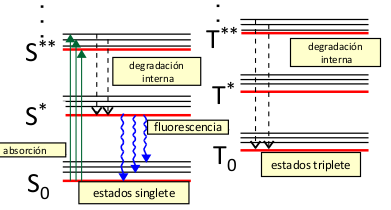
\includegraphics[scale=0.7]{EsquemaNivelesFIbras.png}
\caption{\textbf{Figura 2}.- Esquema de niveles energéticos de un material centelleador ~\cite{asignatura}
}
\end{figure}

Donde los estados S representan singletes y los estados T tripletes. Cuando la radiación ionizante, en nuestro caso los electrones procedentes del tritio, atraviesa el centelleador sus átomos y/o moléculas absorben su energía produciendose una excitación de los mismos. 

Posteriormente estos se desexcitan, en primer lugar desde niveles superiores hasta el nivel S* o $T_0$ por degradación interna (en un tiempo del orden del ps) y seguidamente del S* hasta $S_0$ (en un tiempo del orden del ns). En esta segunda desexcitación emitien fotones cuyo rango de longitud de onda puede ir desde el ultravioleta hasta el infrarrojo [100-800]nm dependiendo de la distancia existente entre estos niveles energéticos. Estos fotones son los que se conocen como fluorescencia y es lo que se utiliza habitualmente como señal de respuesta de un material centelleador (figura 8).

Hay que tener en cuenta que las fibras centelleadoras son transparentes a los fotones que se encuentran en la longitud de onda de su emisión ya que, de lo contrario, tendríamos una nueva reabsorción de los fotones emitidos antes de ser detectados por el contador de fotones, situación indeseada.

Los materiales centelleadoras presentan una muy buena linealidad con la energía de la radiación incidente a partir de una energía mínima que determina la sensibilidad del material centelleador. Teniendo en cuenta que el SiPM también presenta una muy buena linealidad con la señal recibida esperamos obtener una señal de nuestro detector que presente una buena linealidad con la energía que pretendamos medir.

Por lo general estos materiales centelleadores producen señales bastante rápidas en comparación con otros tipos de detectores. Utilizamos fibras centelleadoras orgánicas ya que estas son 2 o 3 órdenes de magnitud más rápidas que las inorgánicas,  en concreto las fibras que utilizaremos presentan un tiempo de decaimiento de 3,2 ns~\cite{datasheet}. Estas poseen un índice de refracción de $1.6$, parámetro fundamental a la hora de transportar eficientemente la luz.

Además debe de ser capaz de producir el mayor número de fotones por unidad de energía para poder tener un mayor detalle de la señal medida. Las fibras BCF-12 son capaces de producir 8000 fotones por MeV de la radiación incidente. Las fibras BCF-12 presentan una eficiencia de fotodetección teórica de 3.4\% ~\cite{datasheet}

Para manipular las fibras se vio necesario la utilización de guantes de latex ya que el propio tacto  del personal encargado del tratamiento de las fibras las ensuciaban y, por extensión, la propagación de la luz se veía afectada.

Para poder cortar las fibras centelleadoras de forma opticamente aceptable se diseño y construyo una guillotina~\cite{Alberto}~\cite{anguloytiempo}~\cite{dependencias}~\cite{tesisfibras} adecuada la cual puede verse reflejada en la figura tres:

\begin{figure}[htb]
\centering
{
%\subfloat[Espectro de emisión]
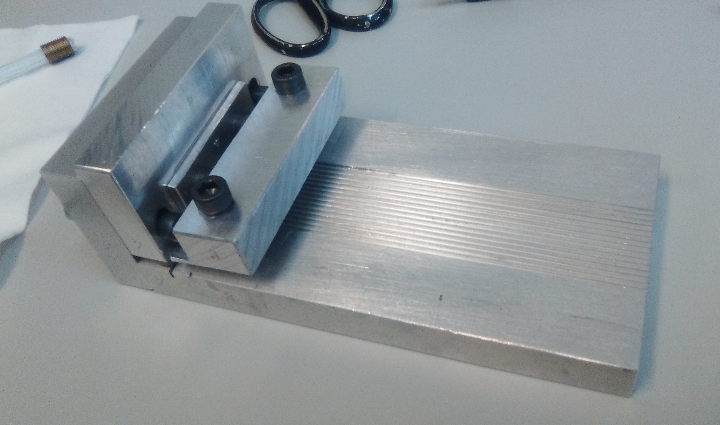
\includegraphics[scale=0.3]{Guillotina1.png} 
}
{
%\subfloat[Espectro de emisión]
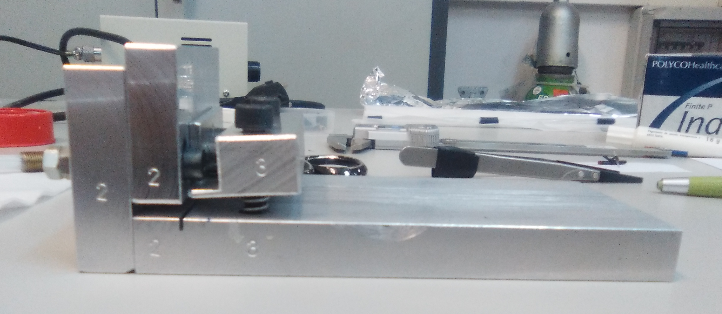
\includegraphics[scale=0.3]{Guillotina2.png} 
}
\caption{\textbf{Figura 3}.-Guillotina}
\end{figure} 

En la figura derecha se puede apreciar que la guillotina disponía de dos piezas independientes (marcadas con los número 2 y 3) las cuales estaban suspendidas por muelles. Para sujetar y cortar cada una de las fibra había que pulsar las piezas 3 y 2 respectivamente. 

También puede apreciarse que la guillotina dispone de 14 rieles cuadrados los cuales servían para sujetar cada una de las fibras y, así, obtener un corte limpio y perpendicular. Aunque la guillotina tenía la posibilidad de realizar cortes simultaneos sobre varias fibras centelleadoras siempre se realizaron cortes sobre una única fibra. De esta forma asegurábamos un mejor acabado.

Se estuvo probando con varios tipos de cuchilla (de distinto grosor y tamaño) y se acabo viendo que una cuchilla típica de afeitar era suficiente. Hay que tener en cuenta que, para un corte más efectivo se introdujo en la disposición de la cuchilla una lijera inclinación~\cite{Alberto}~\cite{anguloytiempo}. 

En la figura cuatro izquierda se puede ver (con ayuda de un microscopio) la cara de una fibra recien cortada. En esta podemos apreciar que, aunque presenta una cabado realmente bueno (sin roturas ni deformaciones) si encontramos que la cara de la fibra se encuentra lijeramente dañada y esto afectaba a la propagación de la luz. La forma de subsanar esto fue pulir cada una de las caras de las fibras. En la parte derecha de la misma figura podemos observar una foto con la misma fibra trás el proceso de pulido. Podemos comprobar que el simple hecho de pulir las caras de las fibras nos permite obtener fibras con acabado ópticamente aceptable~\cite{Alberto}~\cite{manual}.

\begin{figure}[htb]
\centering
{
%\subfloat[Espectro de emisión]
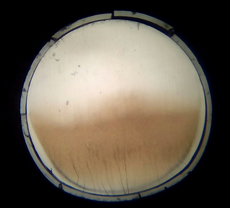
\includegraphics[scale=0.5]{SinPulir.png} 
}
{
%\subfloat[Espectro de emisión]
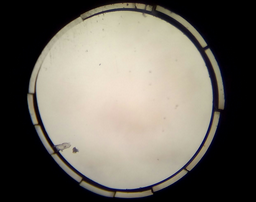
\includegraphics[scale=0.5]{Pulida.png} 
}
\caption{\textbf{Figura 4}.-Cara fibras}
\end{figure} 

Hay que notar en la figura que el clad aparece roto. Se vío que esto era una característica inevitable del proceso de cortado. Sin embargo pudo observarse que este únicamente se encontraba en el extremo final de la fibra por lo que, la utilización de grasa óptica (marca Saint-Global) para acomplar esta al contador de fotones solucionaba el problema.

Seguidamente, con las fibras ya cortadas, simplemente se utilizo un pegamento óptico (marca Saint-Global), especialmente diseñado para materiales centelleadores, para pegarlas entre ellas y obtener, de esta forma, un bunch de fibras. Para que su acabado fuese suficientemente rígido se utilizó un aro metálico en cada uno de los extremos según la figura cinco.

\begin{figure}[htb]
\centering
{
%\subfloat[Espectro de emisión]
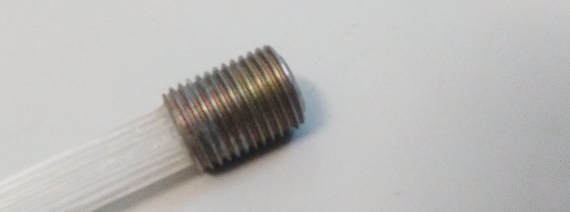
\includegraphics[scale=0.3]{arometalico.png} 
}
{
%\subfloat[Espectro de emisión]
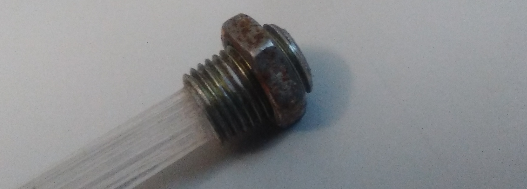
\includegraphics[scale=0.3]{arometalicoconrosca.png} 
}
\caption{\textbf{Figura 5}.-Aro metálico}
\end{figure} 

En la figura cinco derecha puede apreciarse que este mismo aro disponía de una arandela la cual se utilizaba para una completa sujeción al prototipo.

Finalmente, cuando se había secado el pegamento, volvíamos a pulir cada una de las caras del bunch de fibras con el objetivo de obtener una cara total plana (todas las fibras al mismo nivel) para obtener el mejor acomplamiento con el contador de fotones (ya sea SiPM o PMT). En la figura seis podemos observar un buch de fibras totalmente acabado.

\begin{figure}[htb]
\centering
{
%\subfloat[Espectro de emisión]
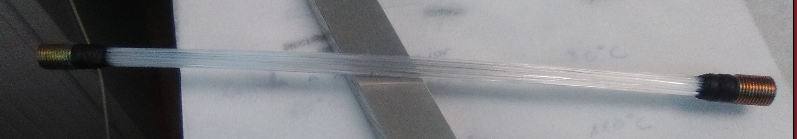
\includegraphics[scale=0.3]{bunchfibras.png} 
}
{
%\subfloat[Espectro de emisión]
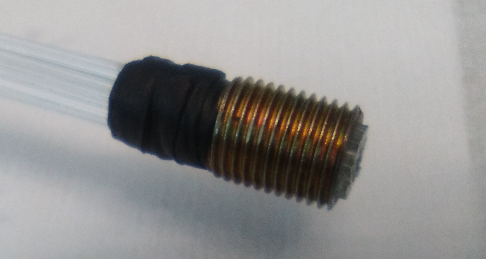
\includegraphics[scale=0.3]{bunchfibras1.png} 
}
\caption{\textbf{Figura 6}.-Bunch fibras}
\end{figure} 

Este bunch construido disponía de 35 fibras ya que era el mayor número de fibras que cabían en el interior del aro metálico y tenía una extensión máxima de aproximadamente 25 cm, extensión acorde con el prototipo. En la figura seis derecha podemos apreciar la cara final pulida perfectamente plana. Hay que tener en cuenta que cualquier irregularidad inferior al milímetro en la cara final de bunch era subsanada por el hecho de utilizar grasa óptica para acoplar el bunch de fibra al contador de fotones.


\newpage
\section{Calibración de los fotomultiplicadores de silicio (SiPM)} \label{sec:ch02}
El siguiente paso consistía en leer estos fotones de centelleo. Para ello una de las alternativas que contempla nuestro estudio es la utilización de un fotomulitplicador de Silicio, de ahora en adelante SiPM. El SiPM es un dispositivo de detección de radiación relativamente nuevo en el mercado que surge como alternativa al tubo fotomultiplicador. Este consiste en un array bidimensional formado por multiples pixels independientes y alimentados en paralelo (mismo voltaje operacional para cada uno) a un voltaje tal que les permita estar en modo Geiger. Cada uno de los pixels actua como un APD (fotodiodos de avalancha)~\cite{TFMSiPM2}.

Cuando detectan un foton estos pixels producen una cascada de pares electrón hueco que pasará a formar parte de la señal del sistema de detección, la cual estará formada por la suma de las señales de cada pixel que han detectado un fotón para cada instante de tiempo. Idealmente cada pixel únicamente puede detectar un fotón. Dado que poseen una alta eficiencia de fotodetección los SiPM son utilizados como contadores de fotones, especialmente para señales débiles.

Debido a ello presenta una serie de propiedades distintas a los convencionales tubos fotomultiplicadores que lo hacen ideal para unas situaciones y no tanto para otras, como por ejemplo su tamaño compacto, inmunidad a campos magnéticos, electrónica sencilla, alta eficiencia de detección de fotones (especialmente adecuado para nuestro experimento), buena linealidad, dependencia con la temperatura, alta ganancia a menor voltaje de alimentación y, por extensión, menor consumo, tiempo de respuesta corto y, por extensión, buena resolución temporal~\cite{AMFNP}.

Hay que tener en cuenta que los SiPM son detectores de estado sólido y, por extensión, presentan ruido térmico, ruido que se verá amplificado por el hecho de estar operando en modo Geiger. Este ruido es denominado corriente oscura (Dark counts) y su forma se ve reflejada en la siguiente figura:

\begin{figure}[hbtp]
\centering
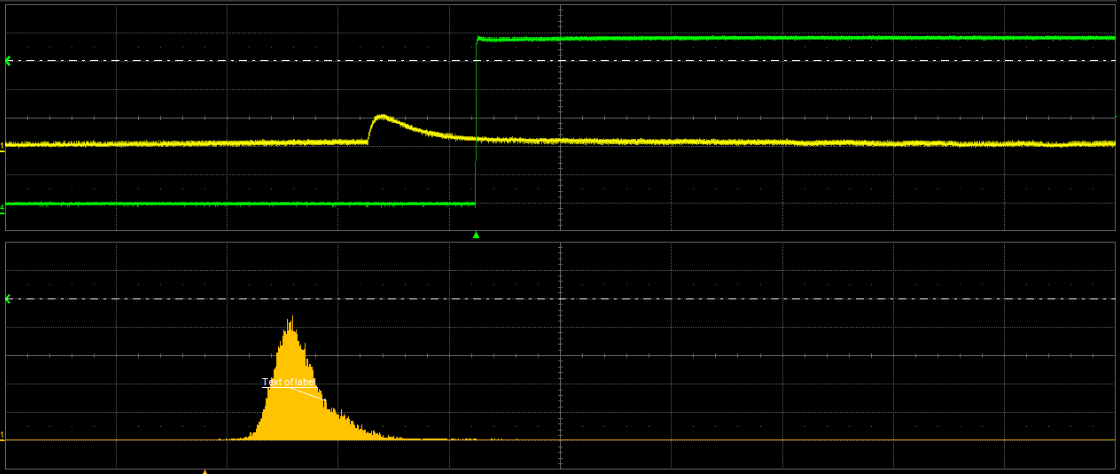
\includegraphics[scale=0.2]{pedestal.png}
\caption{\textbf{Figura 7}.- Dark counts}
\end{figure}

Cuando trabajemos con detectores de estado sólido debemos trabajar en condiciones de voltaje operacional y temperatura óptimas para poder medir con el detector ya  que, estas cuentas oscuras dependen de estas magnitudes y pueden llegar a ser tan numerosas que absorban por completo la señal del sistema. También podemos reducir su importancia sobre la medida con ayuda de triggers, por ejemplo, medir únicamente cuando la señal de entrada del sistema este activa (si se conoce este intervalo de tiempo). En cualquier caso siempre se deberá realizar una medida del pedestal (sin señal de entrada) para tener en cuenta el número y características de los eventos que van a contribuir a la señal sin proceder de la misma y utilizar esta información para el posterior análisis. 

En esta sección nos proponemos desarrollar un método de compensación para las variaciones de la ganancia de un fotomultiplicador de silicio derivadas de la temperatura a partir de variaciones derivadas del voltaje de alimentación del SiPM (voltaje de desertización), de ahora en adelante llamado voltaje operacional. 

En concreto utilizaremos el modelo S13360-1375CS de hamamatsu. Se ha elegido este modelo ya que presenta una eficiencia de fotodetección máxima entorno a los $450~\nm$, que corresponde aproximadamente a la longitud de onda del azul, $435~\nm$ y, en concreto, se asemeja bastante con el máximo de la energía reemitida por las fibras centelleadoras BCF-12, $435~\nm$, encargadas de detectar la radiación $\beta$ del agua tritiada en nuestro experimento como puede apreciarse en la siguiente figura. Con esto conseguiremos que la señal sea tan grande como sea posible, algo fundamental ya que, como ya se ha mencionado, una de las principales dificultados del experimento es que estamos intentando extraer una señal muy pequeña.

\begin{figure}[htb]
\centering
{
%\subfloat[PDE]
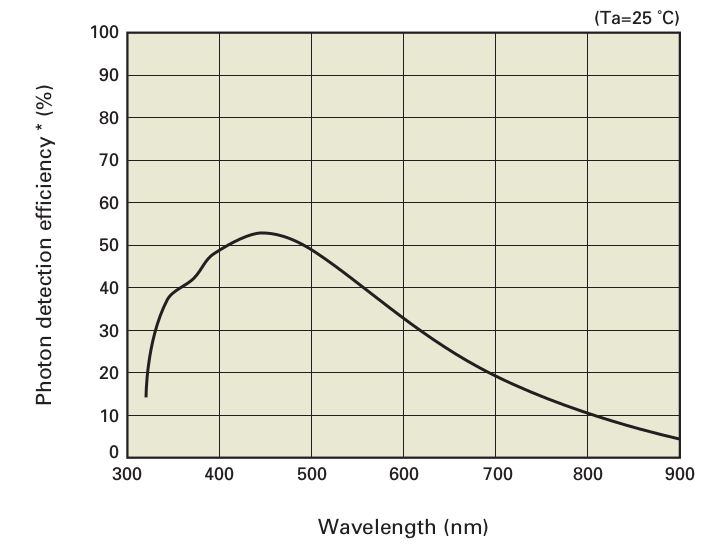
\includegraphics[scale=0.3]{PED.png} 
}
{
%\subfloat[Espectro de emisión]
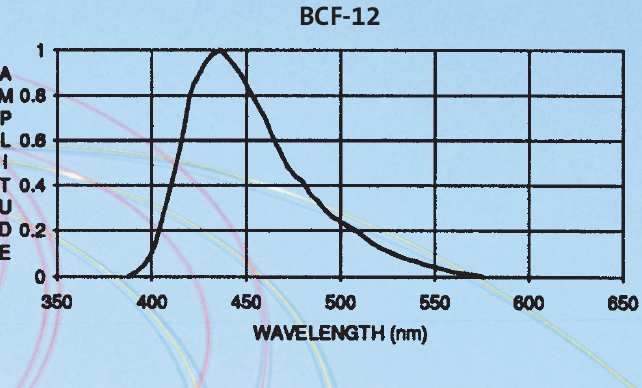
\includegraphics[scale=0.35]{EmisionBCF12.png} 
}
\caption{\textbf{Figura 8}.-PDE del SiPM~\cite{datasheet SiPM} y espectro de emisión de las fibras~\cite{datasheet} respectivamente}
\end{figure}

La forma de abordar este método de compensación de la ganancia ha sido el siguiente:
\begin{enumerate}
\item {} 
Por un lado se ha realizado una calibración de la ganancia frente a la temperatura obteniendo su relación de dependencia. Para ello se ha necesitado la utilización de un sistema de control de temperatura. En concreto se ha utilizado un sistema de la marca DYCOMETAL, (modelo CCM 81) que permite controlar temperatura y humedad relativa con una precisión de $0.1$ grados  y  $0.5$\% respectivamente.

\item {} Por otro lado se ha realizado una calibración de la ganancia frente al voltaje operacional obteniendo su relación de dependencia. Para obtener este voltaje operacional se ha utilizado un electrómetro de la marca KEITHLEY, en concreto el modelo 6517B, el cual presenta una resolución inferior al mV, más que suficiente para considerar este totalmente constante ya que se necesitan mayores modificaciones para que estas sean apreciables en la ganancia.

\item {} Finalmente, a partir de estas dos dependencias determiandas, se ha obtenido la ecuación de dependencia entre voltaje operacional y temperatura que nos determine una ganancia constante  y se ha realizado un test de comprobación para esta relación.
\end{enumerate}

El objetivo final de este estudio será mantener la ganancia del fotomultiplicador de silicio constante ante variaciones involuntarias de la temperatura a partir de variaciones voluntarias con el voltaje operacional. Esta es una correción fundamental para el objetivo final del detector ya que de lo contrario (no) obtendríamos alertas de fugas de tritio cuando estas no (si) han ocurrido, cuando, en realidad, lo único que ha ocurrido ha sido una modificación de temperatura.
	\subsection{Equipo y montaje experimental}
	Para llevar a cabo esta caracterización de los SiPM se ha necesitado de cierta instrumentación la cual se especifica a continuación:

\begin{enumerate}
\item {} En primer lugar se necesitaba una \textbf{cámara de control de temperatura}. 
\newline
Dado que la cámara existente en el laboratorio del IFIC no estaba configurada tuvo que utilizarse la camara que se encontraba en el IFIMED. Esta cámara (marca DYCOMETAL, modelo CCM 81) se ve reflejada en la figura 9 izquierda.

Este sistema dispone de un panel de control con el que poder especificar la temperatura y humedad a la que queremos trabajar en el interior de la cámara. Sin embargo, para asegurar el correcto funcionamiento de la cámara debiamos trabajar siempre en la zona 1 de acuerdo al diagrama de fases existente en la ficha técnica de la cámara, mostrado en la figura 9 derecha. Posee un interior metálico que nos permite una rápida estabilidad ante posibles cambios de las condiciones en su interior y, además, actua a modo de jaula de Faraday. 

\begin{figure}[htb]
\centering
{
%\subfloat[Espectro de emisión]
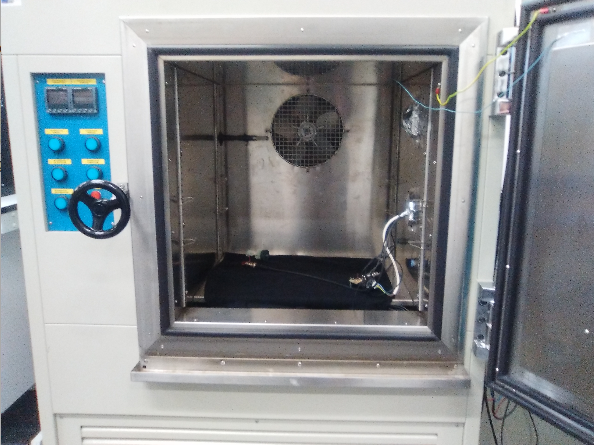
\includegraphics[scale=0.3]{InteriorTemperatura.png} 
}
{
%\subfloat[Espectro de emisión]
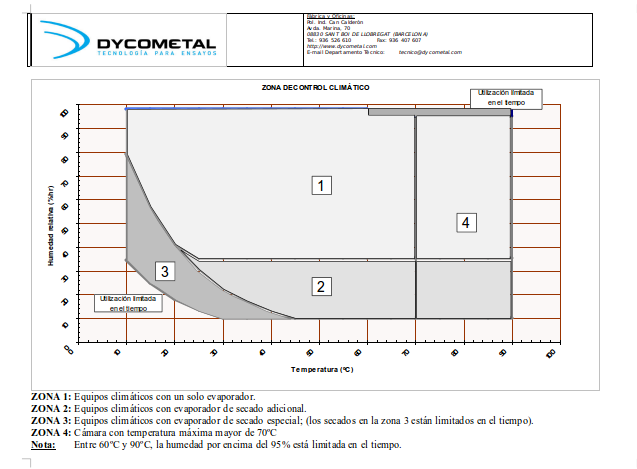
\includegraphics[scale=0.3]{FichaTecnica.png} 
}
\caption{Sistema de control de temperatura y diagrama de fases~\cite{dycometal}\label{sistematemperatura}}
\end{figure}

Su incertidumbre se encontraba en 0.1 grados para la temperatura y 0.5\% para la humedad relativa. Estas incertidumbres se determinaron observando la oscilación  máxima en la pantalla del panel de ambos parámetros tras llegar a la estabilidad en el interior de la cámara.

En el interior de esta cámara se encontraba nuestra fuente que proporcionaba la señal de entrada del sistema que pretendíamos medir con el SiPM, el propio SiPM, la tarjeta de conversión intensidad-voltaje y cableado que hacía posible la interacción con estos dispositivos. Además hay que tener en cuenta que esta cámara no actuaba como caja negra, por lo que para conseguir reducir la posible entrada de luz del exterior se taparon todas las posibles fisuras del sistema con cinta metálica y, ademas, se cubrió el experimento con una tela negra especial. Con todo esto conseguiamos reducir el background del sistema hasta un nivel adecuado.

\item {} En segundo lugar se necesitabamos instrumentos nos permitiesen alimentar tanto el SiPM como la tarjeta de conversión intensidad-voltaje. Se utilizo  un \textbf{electrometro} (marca KEITHLEY, modelo 6517B) para alimentar el SiPM y un \textbf{generador de tensión} (marca ISO-TECH, modelo IPS-4303) para alimental la tarjeta de conversión.

Se utilizo el electrómetro para el SiPM ya que este dispone de rango de voltajes mayor, necesario para alimentar al SiPM. Por el contrario, el ISO-TECH solo dispone de una tensión máxima de 30V insuficiente para alimentar al SiPM pero suficiente para alimentar la tarjeta. Poseen una resolución inferior inferior al milivoltio e inferior a 0.1 voltios respectivamente, suficiente para considerarlos constantes ya que las ganancias que dependen de estos (ganancia del SiPM y de la tarjeta respectivamente) necesita variaciones superiores para modificarse de forma apreciable.

\item {} En tercer lugar se necesitaba una \textbf{fuente} que simulase la emisión de los fotones de la fibra centelleadora. 
\newline
Se utilizo un \textbf{diodo LED} (de la empresa Roithner Laser technik) que emitía fotones con una longitud de onda de 435 nm ~\cite{datasheetLED}, correspondiente al azul. Este es la longitud de onda que necesitabamos en nuestro experimento para calibrar el SiPM ya que corresponde a la longitud de onda a la cual el espectro de emisión de las fibras centelleadoras BCF-12 tiene su máximo.

%\newpage
\item {} En cuarto lugar, para alimentar este diodo LED, se necesito un \textbf{generador de pulsos} (marca Agilent, modelo 33250A). Este generador de señales nos permite especificar la forma del pulso que pretendemos proporcionar y sus características. Este tenía que ser capaz de formar un pulso suficientemente estrecho para que el SiPM detectase unos pocos fotones. 

En concreto alimentaremos el diodo LED con un pulso cuadrado. Los parámetros que nos permite especificar el generador de señales para un pulso de esta forma son frecuencia (o periodo), high level (o amplitud), low level, offset, anchura del pulso y tiempo de decaimiento. Para nuestro estudio los valores de estos parámetros que nos daban un mejor resultado desde el punto de vista experimental fueron una frecuencia de 20 Hz, high level de 2.275 V, low level de 1 V, offset de 1.638 $V_{dc}$, anchura del pulso de 12 ns y tiempo de decaimiento de 5 ns.

Este generador de señal nos proporciona una segunda señal denominada señal de sincronización la cual podemos utilizar como trigger para determinar el instante de tiempo en el que se activa la señal.

\item {} En quinto lugar utilizamos un \textbf{SiPM} para detectar los fotones emitidos por el LED. En concreto se utilizo el modelo S13360-1375CS de hamamatsu, que es un fotomultiplicador cerámico de silicio que presenta una ganancia teórica de $G=4 \cdotp 10^6$ y una eficiencia de fotodetección teórica del 50\% a 25 grados y $V_{ov}=V_{op}-V_{bd}=3V$. Este tiene un rango espectral de [270-900] nm~\cite{datasheet SiPM}.

Esta compuesto por un total de 285 pixels de 75 $\mu m$ cada uno dando lugar a una superficie total activa de 1.3x1.3 $mm^2$ frente a su superficie total que es de 6x5 $mm^2$. Puede verse reflejado en la figura 10 izquierda~\cite{datasheet SiPM}. 

\item {} Hay que tener en cuenta que el SiPM nos proporciona un pulso de intensidad a la salida y  necesitamos convertir este en un pulso de voltaje para, de esta forma, poder introducirla al osciloscopio para realizar el posterior análisis. Para ello emplearemos en sexto lugar una \textbf{tarjeta conversora} de intensidad en voltaje que puede verse reflejada en la figura 10 derecha. 

\begin{figure}[htb]
\centering
{
%\subfloat[Espectro de emisión]
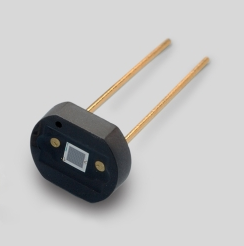
\includegraphics[scale=0.4]{SiPM.png} 
}
{
%\subfloat[Espectro de emisión]
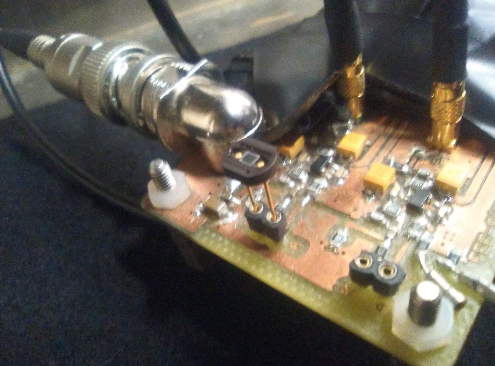
\includegraphics[scale=0.4]{tarjeta.png} 
}
\caption{SiPMs y tarjeta de conversora intensidad-voltaje\label{TarjetaSiPM}}
\end{figure}

\item {} Finalmente vimos que, únicamente alimentando la tarjeta, antes de alimentar el SiPM y la led, obteníamos una perturbación externa a nuestro experimento. Esta se presenta en la figura 11. 

\begin{figure}[hbtp]
\centering
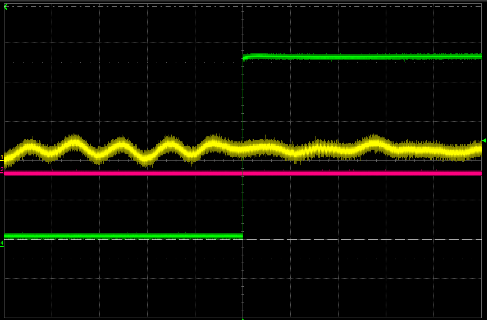
\includegraphics[scale=0.4]{ruido.png}
\caption{Ruido electrónico\label{Ruido}}
\end{figure}

Se intento caracterizar esta señal de perturbación ajena a nuestro experimento y, a priori, de origen desconocido. Tenía una amplitud máxima de 4 mV y una frecuencia bastante irregular entorno al MHz. Finalmente se vio que era debido por una parte a la emisión producida por la antenas de radiotelevisión valenciana y, por otra parte, de las distintos intrumentos electrónicos conectados a la red eléctrica del IFIC, ya que esta posee una toma a tierra bastante irregular. 

Con la presencia de este ruido no podíamos realizar medidas ya que introducía una componente de ruido tal que estropeaba por completo el resultado de la medida. Con el fin de solucionar este problema se dispuso de un \textbf{filtro pasa banda} (GUARD LCD2 650 AP) para eliminar este ruido.

\item {} Finalmente, como se ha mencionado anteriormente, necesitamos una \textbf{manta negra} especial que apantallase la entrada de fotones del exterior, ya que el sistema de control de temperatura no actuaba como caja negra.

Una alternativa podría haber sido introducir una caja negra en el interior del sistema de control de temperatura y introducir el diodo Led, el SiPM y la tarjeta en su interior. Sin embargo de esta forma no conseguimos un control de la temperatura y humedad en su interior.

\end{enumerate}

	
	\subsection{Calibración tarjeta}
	La tarjeta empleada en el sistema, la cual puede apreciarse en la figura diez, es una tarjeta reciclada un un proyecto anterior. La necesidad de esta, como se ha comentado anteriormente, reside en que la señal de salida de un SiPM es una señal de intensidad y el osciloscopio únicamente puede trabajar con señales de voltaje. Por tanto, para poder analizar esta señal es necesario utilizar una tarjeta conversora de intensidad en voltaje. Esta consiste de dos entradas donde podemos conectar dos SiPM distintos. La tarjeta contine un circuito similar al de la siguiente imágen para cada SiPM:

\begin{figure}[hbtp]
\centering
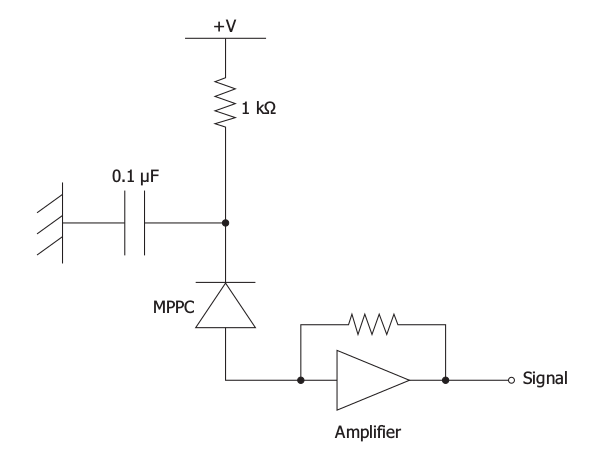
\includegraphics[scale=0.4]{CircuitoTarjeta.png}
\caption{\textbf{Figura 12}.- Circuito de una tarjeta tipo}
\end{figure}


Es una tarjeta del departamento de electrónica, cuyos ingenieros nos han informado que posee una ganancia de $G=110$. Este será el valor que utilizaremos en el análisis posterior para calcular la ganancia de los SiPM.

%Dado que no conocemos su incertidumbre consideraremos este valor como un valor sin error. Esto nos conducirá a obtener una subestimación de la incertidumbre de la ganancia de los SiPM. Sin embargo esto no tiene mayor importancia ya que será un factor constante que afectará por igual a todas las medidas y no estamos buscando determinar la ganancia de los SiPM sino únicamente sus dependencias con el voltaje y la temperatura. 
	
	\subsection{Análisis de datos}
	En resumen, en nuestra prueba de calibración de los SiPM tenemos una caja que actuará como jaula de faraday, con temperatura y humedad controlada y apantallada en lo posible de la luz del exterior. 

En su interior tendremos un diodo LED que emite fotones a $\lambda=435~\nm$, un SiPM, el cual emitirá un pulso de intensidad cada vez que detecte uno o más de estos fotones con cada uno de sus pixels y una tarjeta que convertirá este pulso de intensidad en un pulso de voltaje. Finalmente llevamos este pulso de voltaje a un osciloscopio (marca TELEDYNE LECROY, modelo WwaveRunner 625Zi) para poder ser analizado. 

Una vez en el osciloscopio, la señal que recibíamos cuando se encendía el diodo LED será similar a la de la señal superior de la figura trece (amarilla)~\cite{inftec}, el la cual se a activado el modo persistencia del osciloscopio con el objetivo de comparar señales de distintas alturas. Estas señales corresponden a distinto número de pixels activados en cada instante de tiempo ya que, como hemos dicho anteriormente, la señal de salida del sistema es la suma de las señales de cada pixel que se ha activado. Esta se encuentra superpuesta a la señal de sincronización del generador de señales (verde) que nos muestra cuando se ha encendido el diodo LED y que, por tanto, actua como trigger.

El objetivo ahora es calcular la ganancia del sistema. Dado que únicamente existen dos ganancias en el sistema (SiPM y tarjeta) y hemos medido la ganancia de la tarjeta en la sección anterior, determinando la ganancia total podremos determinar de forma aproximada la ganancia del SiPM. 

\begin{equation}
G_{tot}=G_{SiPM} \cdotp G_{card} \longrightarrow G_{SiPM} = \frac{G_{tot}}{G_{card}}
\label{ganancias}
\end{equation}

Para medir la ganancia total simplemente realizamos una integral del area de cada uno de los pulsos de salida del sistema y conservamos el resultado en un histograma. De esta forma lo que estamos consiguiendo es un histograma de las cargas de los pulsos. La ventana temporal sobre la que se integra es aproximadamente una división, que equivale a $500~\ns$. Esta se ajusta con bastante precisión al pulso, algo muy importante para evitar la introducción de background.

Dado que idealmente el pulso de cada pixel es igual, el histograma que estamos obteniendo deberían ser deltas de dirac equiespaciadas. Sin embargo hay que tener en cuenta que la cascada que produce cada uno de estos fotones detectados en cada pixel esta sometido a fluctuaciones estadísticas. Además los propios instrumentos de medidas empleados tienen una incertidumbre inherente. Hay que tener en cuenta que tambień tenemos distintas fuentes de background, como dark counts (ruido térmico), fotones de luz del exterior, etc. 

Como resultado de todo esto, lo que obtendremos seran un conjunto de gaussianas equiespaciadas. En la figura trece inferior puede verse el resultado de una toma de datos de 25000 eventos a 25 grados, 60\% de humedad y $V_{ov}=3V$

\begin{figure}[hbtp]
 \centering
 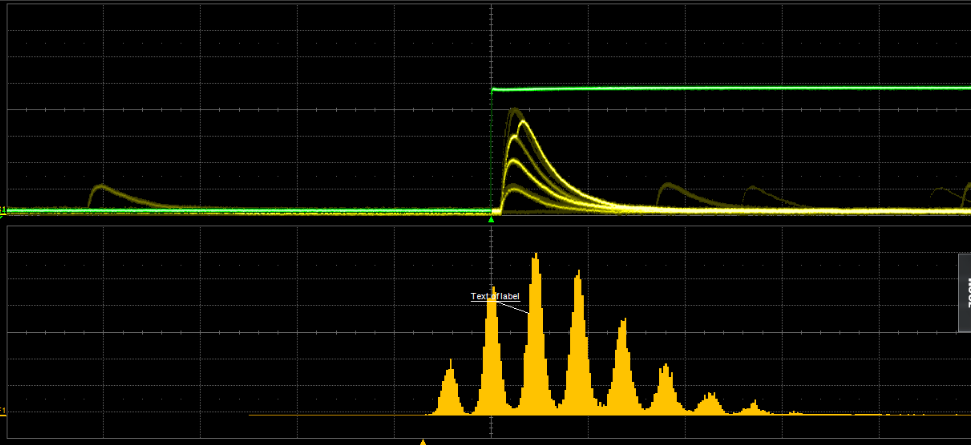
\includegraphics[scale=0.4]{Analisis.png}
 \caption{\textbf{Figura 13}.- Análisis}
 \end{figure}

Donde cada uno de estos picos corresponde a la carga de sucesivos número de pixels activados (uno, dos, etc.). El primer pico no debe tenerse en cuenta en el análisis ya que este corresponde al pedestal (cero pixels activados). Su origen es debido a la existencia de las cuentas ocuras.
 
Ahora únicamente desarrollamos una macro en ROOT (programa de análisis de datos desarrollado por el CERN) que, utilizando la librería TSpectrum (librería especialmente diseñada para el análisis de histograma) nos permita obtener la ganancia del sistema. Su forma de proceder es la siguiente:
\begin{enumerate}
\item {} Primero la macro lee el fichero de datos y lo guarda en una variable de tipo histograma. La macro se detiene cuando no encuentra más valores para leer.

\item {} A continuación, a partir de una función de la librería TSpectrum, busca en este histograma y devuelve el número de gaussianas que ha encontrado y su posición.

\item {} Ahora ajusta todos los datos del histograma a una recta y solo se queda con las gaussianas, cuya norma sobrepasa en altura a esta recta. El objetivo de este paso es que, en casos muy concretos (temperatura alta o luz del laboratorio encendida) tenemos mucho ruido y, aparece un fondo el cual, el programa ajusta a una gaussiana y, por extensión, calcula la ganancia de manera incorrecta. Un ejemplo de esto se muestra en la figura catorce.

\begin{figure}[hbtp]
\centering
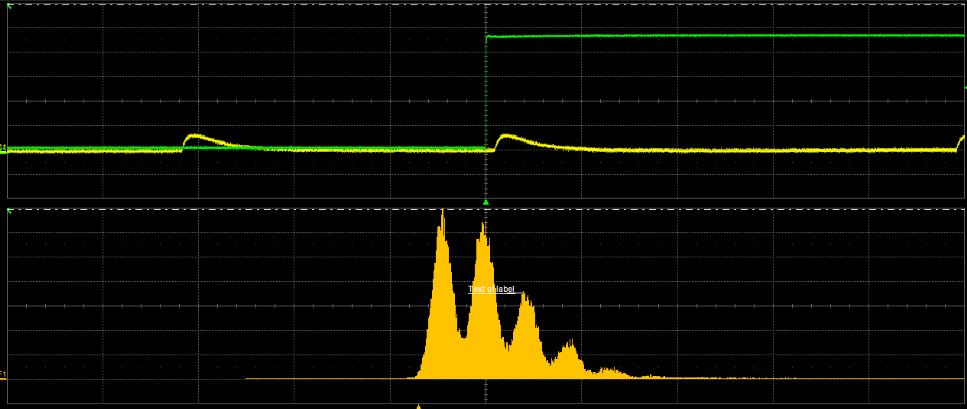
\includegraphics[scale=0.4]{fondogaussiano.png}
\caption{\textbf{Figura 14}.- Espectro con mucho fondo}
\end{figure}

\item {} Seguidamente, ajustamos el espectro a una recta mas una suma de n gaussianas, donde n es el número de gaussianas que superan la recta (calculado en el paso anterior). La necesidad de utilizar una recta es debido a que siempre vamos a tener dark counts y otro tipo de bakcground que se verán reflejados en una linea base en el histograma como puede verse en la figura trece. Podemos apreciar en la figura quince que el ajuste (linea roja) es relativamente bueno. Para poder ver hasta que punto nuestro ajuste es aceptable aplicamos el test $\chi^2$, donde se ha obtenido un resultado de $\frac{\chi^2}{ndf}=\frac{1276}{223}\approx 5.72$. Vemos que efectivamente el ajuste se realizado con gran precisión.

\begin{figure}[hbtp]
\centering
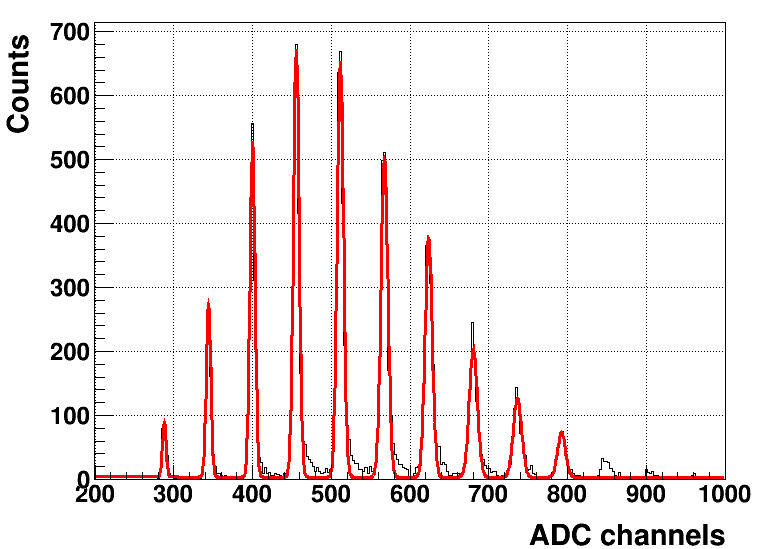
\includegraphics[scale=0.4]{AjusteEspectro1.png}
\caption{\textbf{Figura 15}.- Ajuste de la macro de ROOT sobre un espectro}
\end{figure}

\item {} Dado que se ha observado que, aun con el tercer paso, existen situaciones límites en que el background sigue superando esta recta, se ha incluido un paso en la macro en la cual se acepta por teclado uno a uno los picos que serán utilizados en el análisis. Además la macro calcula la resolución de cada gaussiana y la resolución total, obtenida a partir de la suma cuadrática de la resolución de cada gaussiana. Los valores habitualmente encontrados en los análisis se encuentran sobre 1.5\% y 5\% respectivamente, valores más que aceptables.

\item {} Finalmente la macro los ordena según su posición en el espectro y calcula la ganancia por dos caminos:
	\begin{enumerate}

	\item {} Por un lado se ha calculado la distancia promedio entre sucesivas gaussianas del espectro~\cite{Hueso}.
	\begin{equation} 
	Q = G N_\gamma + Q_0 \longrightarrow \Delta Q= Q_{N_\gamma} - Q_{N_\gamma -1}=G N_\gamma+ Q_0 - G(N_		\gamma -1) - Q_0 = G
	\label{gananciametodo1}
	\end{equation}
	Podemos observar que este cálculo corresponde a la ganancia. Hay que tener en cuenta que se han empleados factores de conversión para convertir la posición del pico (inicialmente en unidades de	tensión, V) en unidades de carga (coulomb). En concreto se ha utilizado el factor $\frac{1}{eR}$, donde R es la resistencia del osciloscopio, 50 $\Omega$ y e es la carga del electrón.
	
	\item {} Por otro lado se ha ajustado a una recta las posiciones horizontales de estas gaussianas en el 	espectro frente a el número de pixels. Esto nos da la siguiente ecuación~\cite{Hueso}:
	\begin{equation}
	Centro\_pico(V) = GeRN_\gamma + k_0
	\label{gananciametodo2}
	\end{equation}
	Donde R y e significan lo mismo. Vemos por tanto que apartir del valor de la pendiente podemos obtener	el valor de la ganancia. La figura dieciseis muestra un ejemplo de ajuste entre posiciones de gaussianas y número de pixels para el caso de 25 grados, humedad de 45\% y $V_{ov}=3V$. Podemos observar que existe	un acuerdo excelente, algo que ocurria prácticamente en la totalidad de los casos. Este gráfico presenta barras de error pero no son apreciables a esta escala.
		
	\begin{figure}[hbtp]
		\centering
		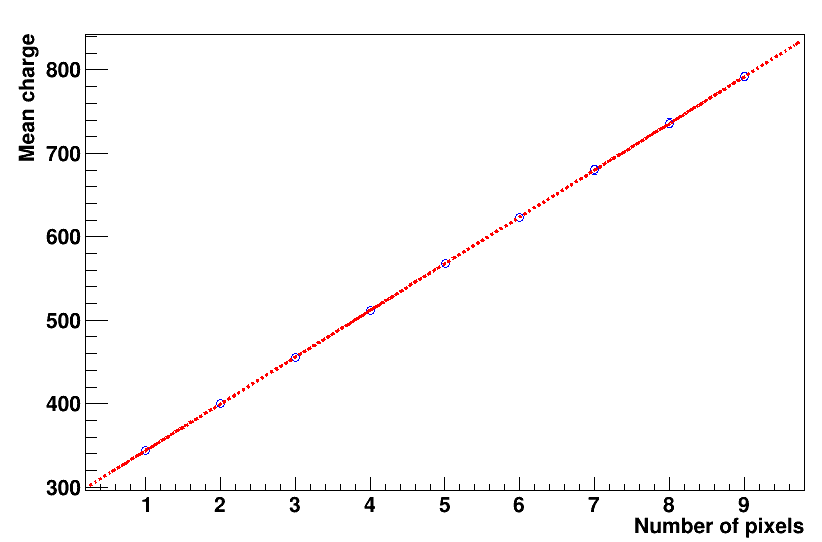
\includegraphics[scale=0.4]{FitPosicionPixels.png}
		\caption{\textbf{Figura 16}.- Ajuste carga de las señales del SiPM frente a nº de pixels encendidos}
		\end{figure}
			
	\end{enumerate}
	
Para este caso concreto las ganancias obtenidas por los dos caminos anteriores son respectivamentente:
\begin{equation}
G_1= 6.38938 \cdot 10^8 \pm 2.15953 \cdot 10^8
\label{gananciatotalmetodo1} 
\end{equation}
\begin{equation}
G_2=7.18235 \cdot 10^8 \pm 6.88392 \cdot 10^6
\label{gananciatotalmetodo2}
\end{equation}
Por extensión, las ganancias del SiPM calculadas por cada camino son (aproximadamente)$\eqref{ganancias}$: 
\begin{equation}
G_1= 5.80853 \cdot 10^6 \pm 1.96321 \cdot 10^6
\label{gananciaSiPMmetodo1}
\end{equation}
\begin{equation}
G_2= 6.52941 \cdot 10^6 \pm 6.258 \cdot 10^4
\label{gananciaSiPMmetodo2}
\end{equation}

donde los errores se han obtenido por propagación. Si comparamos con la literatura~\cite{datasheet SiPM} podemos observar que ambos valores son bastante aceptables con errores relativos de:

\begin{equation}
\sigma_{rel1} \approx 0.0319 = 3.19\%; \qquad \sigma_{rel2} \approx 0.0882 = 8,82\%
\label{erroresgananciasSiPM}
\end{equation}


Dado que, en la practica, las gaussianas no estan perfectamente equiespaciadas debido a errores e incertidumbres consideraremos como más fiable el segundo método ya que se trata de un método más formal, a pesar de tener un error relativo mayor.

Nuevamente se ha aplicado el test $\chi^2$ con el objetivo de comprobar la calidad de nuestro ajuste. Se ha obtenido un resultado de $\frac{\chi^2}{ndf}=\frac{0.05452}{7}\approx 0.008$. Podemos apreciar que ahora hemos obtenido un valor bastante por debajo de la unidad. Este, probablemente, es debido a que se han sobreestimado los errores de las medidas (calculados a partir de las sigmas de las gaussianas del ajuste de la figura 15).

\end{enumerate}
	
	\subsection{Calibración en temperatura}
	Ahora que ya sabemos calcular la ganancia del SiPM a partir de una toma de datos procedemos a determinar la dependencia que presenta el SiPM con la temperatura. En concreto nos interesa determinar el comportamiento de su ganancia cuando varía la temperatura. Para ello realizaremos una serie de medidas a distintas temperaturas y, para cada una de ellas, calcularemos la ganancia a partir del metodo expuesto en el punto anterior.

Nos centraremos en el rango de temperatura entre 15 grados, que es el mínimo que nos permitía llegar el sistema de control de temperatura y 41 grados, que, suponemos, será el límite al que llegará nuestro futuro detector en la práctica. Es decir, este rango de temperaturas será equivalente a las temperaturas a las que estará sometido nuestro detector debido a las condiciones climáticas del lugar. Realizaremos pasos de 2 grados entre cada medida realizando un total de 14 medidas. Únicamente realizaremos medidas de 15000 eventos ya que son más que suficiente para obtener un espectro suficientemente suave. 

Para automatizar este proceso procedemos a desarrollar una macro en ROOT que realice este ajuste. Esta macro se divide en dos partes:
\begin{itemize}
\item{} Por un lado posee un bucle en el que, en cada paso, abre el fichero correspondiente a una temperatura, empezando por la mínima (15 grados) realiza todo el estudio anterior y guarda ganancia y temperatura con sus errores en 4 vectores respectivamente. En cada paso aumenta 2 grados la temperatura y pasa a leer el siguiente fichero.

Hay que tener en cuenta que, como se dijo anteriormente, el sistema de control de temperatura debe de estar en la zona uno del diagrama de fases existente en la ficha técnica. Esto implico que, para medidas inferiores a 27 grados necesitamos aumentar la humedad en un 5\% a cada medida (humedad del 45\% para 25 grados, 50\% para 23 grados, etc.). Esto no tiene mayor importancia ya que se vio que la ganancia del SiPM no se ve afectada de forma apreciable ante modificaciones de la humedad de este tamaño.

La incertidumbre en la temperatura viene dada por la oscilación en el valor de la temperatura observada directamente en el panel de control del sistema. La oscilación observada fue en todo momento de 0.1 grados, una incertidumbre totalmente inapreciable tanto a nivel visual en la gráfica como a nivel de variación de la ganancia.

\item {} Por otro lado, partiendo de estos 4 vectores de dimensión 14 en nuestro caso (igual al número de ficheros que ha leido) que contienen ganancia, temperatura y sus errores de forma ordenada la macro realiza un ajuste lineal. El ajuste obtenido se presenta en la figura 17.

\begin{figure}[hbtp]
\centering
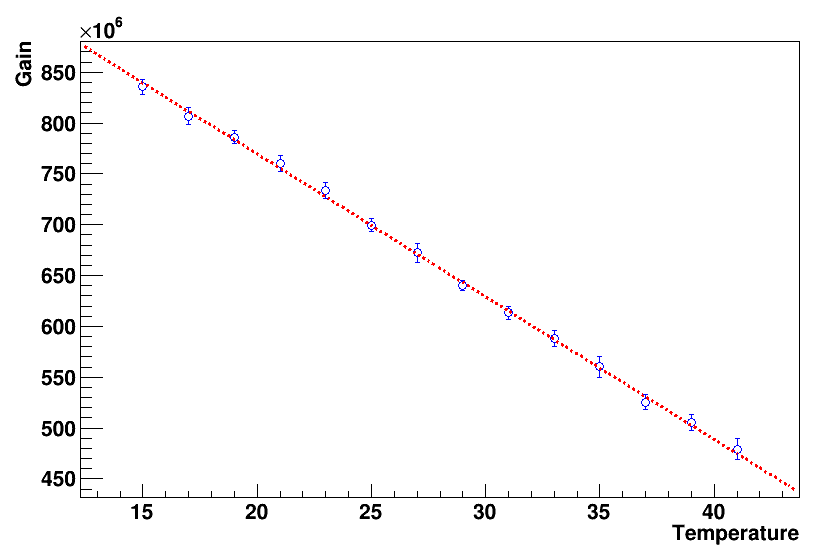
\includegraphics[scale=0.4]{Dependenciatemperatura.png}
\caption{ Ganancia frente a temperatura\label{temperatura}}
\end{figure}

Podemos observar la existencia de un comportamiento lineal casi perfecto en un rango de temperatura de 26 grados. Esta es una propiedad que caracteriza al SiPM, una muy buena linealidad en su comportamiento frente a modificaciones en varias magnitudes. Nuevamente comprobamos la calidad del ajuste a partir del test $\chi^2$ obteniendo un valor de $\frac{\chi^2}{ndf}=\frac{2.937}{12}\approx 0.245$, el cual se trata de un valor relativamente bueno.

En la gráfica encontramos, como esperábamos~\cite{tesisSiPM}, la existencia de un decrecimiento del valor de la ganancia del SiPM a medida que aumenta la temperatura. Esto es debido a que la zona de desertización, que se crea en el SiPM al aplicar un voltaje en inversa y que actura como zona útil de detección de radiación, depende de la temperatura. En concreto, al aumentar la temperatura estamos incrementando la excitación térmica de los portadores de carga pudiendo, de esta forma, invadir esta zona de desertización, reduciéndola su tamaño y, por extensión, la ganancia del SiPM.

La ecuación obtenida en este ajuste $G=aT+b$ toma los siguientes valores: 
\begin{equation}
a=-1.40308 \cdot 10^7 \pm 2.71545 \cdot 10^5~\frac{1}{ºC}
\label{ajustependientetemperatura}
\end{equation}
\begin{equation}
b=1.05001 \cdot 10^9 \pm 7.69711 \cdot 10^6 ~\frac{1}{ºC}
\label{ajusteordenadatemperatura}
\end{equation}


Esta es un resultado importante, no por el valor numérico, sino porque será la base que utilizaremos para conseguir la compensación de la ganancia.
\end{itemize}

	\subsection{Calibración en voltaje de operación}
	De forma totalmente análoga procedemos a determinar el comportamiento del SiPM, en concreto de su ganancia, frente al voltaje operacional. Para ello realizaremos una serie de medidas a distintos voltajes operacionales y, para cada una de ellos, calcularemos la ganancia a partir del metodo expuesto anteriormente. 

Nos centraremos en el rango de voltajes entre el voltaje break down, $V_{BD}= 50.97$ V, que es el mínimo voltaje en valor absoluto a partir del cual nos encontramos en modo Geiger y $V_{BD}+5V$, que, suponemos, será un intervalo suficiente para compensar la ganancia acorde con el intervalo de temperaturas que hemos medido. Realizaremos pasos de 0.2 V entre cada medida realizando un total de 25 medidas. De nuevo unicamente realizaremos medidas de 15000 eventos ya que son más que suficiente para obtener un espectro suficientemente suave.

Para automatizar este proceso procedemos a desarrollar una macro en ROOT que realice este ajuste. Análogamente esta macro poseerá dos partes:
\begin{itemize}
\item{} Por un lado posee un bucle en el que, en cada paso, abre el fichero correspondiente a un voltaje operacional, empezando por el mínimo ($V_{op}=V_{BD}$) realiza todo el estudio anterior y guarda ganancia y voltaje operacional con sus errores en 4 vectores respectivamente. En cada paso aumenta 0.2 V el voltaje operacional y pasa a leer el siguiente fichero. 

En este estudio, a diferencia del estudio de la temperatura, la incertidumbre en el voltaje viene dada por la precisión del electrómetro (milivoltio) ya que el valor era perfectamente estable. Esta, de nuevo es una incertidumbre totalmente inapreciable tanto a nivel visual en la gráfica como a nivel de variación de la ganancia. 

Hay que tener en cuenta que el voltaje operacional posee un error relativo, definido como $\frac{\sigma_x}{x}$ muy inferior al de la temperatura, siendo estos aproximadamente $1 \cdot 10^{-5}$ y $8 \cdot 10^{-3}$ respectivamente. Es decir, las medidas que tomemos en este estudio serán más preceisas.

\item {} Por otro lado, partiendo de estos 4 vectores de dimensión 25 en nuestro caso (igual al número de ficheros que ha leido) que contienen ganancia, temperatura y sus errores de forma ordenada realiza un ajuste lineal. El ajuste obtenido se presenta en la figura dieciocho.

\begin{figure}[hbtp]
\centering
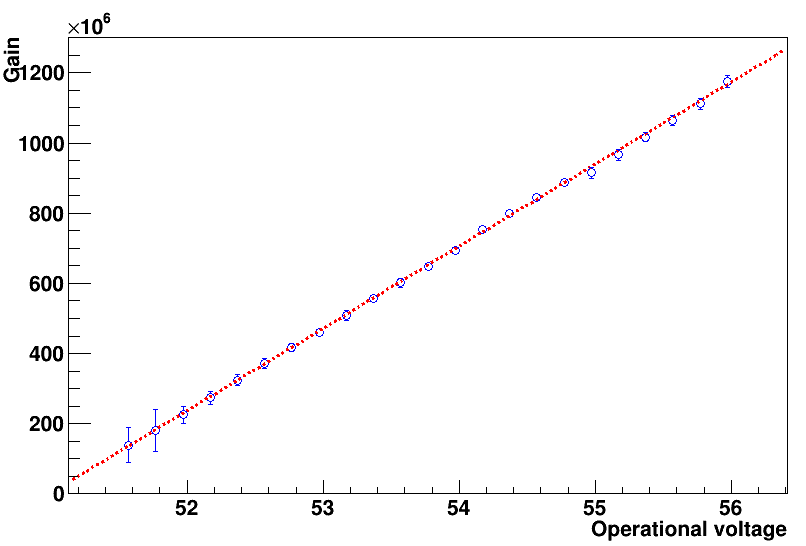
\includegraphics[scale=0.4]{Dependenciavoltaje.png}
\caption{\textbf{Figura 18}.- Ganancia frente a voltaje operacional}
\end{figure}

Podemos apreciar de nuevo la existencia de un comportamiento lineal casi perfecto en un rango de voltaje de 5 voltios. Vemos de nuevo reflejada la propiedad de buena linealidad que caracteriza a los SiPM. En la gráfica podemos notar la existencia de un mayor error en las medidas de voltajes mas bajos (en valor absoluto). Esto es debido a que nos estamos acercando al voltaje break down donde el silicio entra en modo Geiger y el valor de la ganancia empieza a ser distinto de cero. Podemos hachacar este mayor error a que a estos voltajes cercanos a la frontera de cambio de comportamiento, el SiPM todavía no funciona de forma adecuada debido a efectos más sutiles. Este necesita estar totalmente dento del modo Geiger para funcionar perfectamente. Hay que tener en cuenta además que solo se llego hasta el voltaje $V_{op}=51,57$ V debido a que, cuando estamos a valores muy cercanos al voltaje de break down la ganancia sufre un decaimiento exponencial, siendo imposible realizar su medida.

De nuevo comprobamos la calidad del ajuste a partir del test $\chi^2$ obteniendo un valor de $\frac{\chi^2}{ndf}=\frac{7.963}{21}\approx 0.379$, el cual se trata de un valor relativamente bueno.

Podemos observar que, al contrario de lo que ocurría con la temperatura, el valor de la ganancia del SiPM aumenta a medida que aumenta el voltaje operacional. Esto es debido a que a medida que aumentamos el voltaje operacional aumenta la diferencía de potencial en la zona de desertización. De esta forma, por un lado, aumentando la zona de desertización, por lo que los pares electrón--hueco dispondrán de mayor espacio para generar una mayor replicación y, por otro lado, estamos aplicando una mayor tensión sobre los pares electrón-hueco generados al detectar radiación y, por extensión, estos se verán acelerádos más rápidamente. Debido a ello dispondrán de una mayor energía para producir un mayor número de pares electrón-hueco. En resumen ambos procesos contribuyen a aumentar la ganancia del SiPM.

La ecuación obtenida en este ajuste $G=cV_{op}+d$ toma los siguientes valores: 
\begin{equation}
c=2.34123 \cdot 10^8 \pm 2.55246 \cdot 10^6~V^{-1}
\label{ajustependientevoltaje}
\end{equation}
\begin{equation}
d=-1.19368 \cdot 10^{10} \pm 1.38112 \cdot 10^8~V^{-1}
\label{ajusteordenadavoltaje}
\end{equation}

Remarquemos de nuevo la importancia de este resultado, no por el resultado numérico, sino porque es la parte que nos faltaba para poder calcular la compensación de la ganancia.

A demás, a modo de comprobación, podemos obtener el Voltage break down a partir de esta expresión, que se corresponde al voltaje al cual la ganancia es cero (voltage a partir del cual estamos en modo geiger y la ganancia empieza a ser no nula). El voltage calculado es: 
\begin{equation}
G=0=c \cdot V_{BD} +d \longrightarrow V_{BD}=-\frac{d}{c}=50.9852~V
\label{ajustebdv}
\end{equation}

Vemos que este se acerca de forma extraordinaria al voltaje teórico especificado por hamamatsu, $50.97~V$.
\end{itemize}
	
	\subsection{Estabilización de la ganancia}
	Finalmente, con toda esta información, procedemos a desarrollar un protocolo de compensación de la ganancia. Nuestro objetivo es que, ante una modificación de la ganancia debido a una variación involuntaria de la temperatura (por ejemplo debido a variación climatológicas) aplicar de manera voluntaria una variación adecuada en el voltaje operacional que devuelva a la ganancia a su valor inicial.

Como ya se ha explicado la importancia de este estudio de compensación es poder utilizar este sistema a modo de alarma. Dado que este estará expuesto a condiciones climáticas inevitablemente sufrira variaciones de temperatura. Si queremos el detector final sea capaz de avisar en caso de obtener una señal demasiado grande y que esta señal se corresponda a una fuga de tritio necesitamos que el sistema posea una ganancia constante.

Las expresiones que se han obtenido con las dos calibraciones anteriores son:
\begin{equation}
G(V_{op})=cV_{op}+d; \qquad G(T)=aT+b
\label{gananciatotal}
\end{equation}
Esto implica que una variación de la ganancia en cada una de estas magnitudes viene reflejado como:
\begin{equation}
\partial G(V_{op}) = c \partial V_{op}; \qquad \partial G(T) = a \partial T
\label{variacionparcialganancia}
\end{equation}
Finalmente, la variación total de la ganancia ante una variación de ambas magnitudes viene dado por:
\begin{equation}
\partial G_{tot} = \partial G(V_{op}) + \partial G(T)
\label{variaciontotalganancia}
\end{equation}
Por tanto, si queremos que el valor de la ganancia se conserve ante una variación de ambas magnitudes tendremos que conseguir que: 
\begin{equation}
\partial G_{tot} = 0 =  \partial G(V_{op}) + \partial G(T) \longrightarrow \partial G(V_{op}) = -\partial G(T)  
\label{basecompensacion}
\end{equation}
En otras palabras, lo que tenemos que conseguir es producir la misma variación a la ganancia con la modificación del voltaje que la que se ha producido al variar la temperatura. Para determinar esta variarión únicamente sustituimos las expresiones anteriormente obtenidas para cada diferencial de la ganancia:
\begin{equation}
\partial G(V_{op}) = - \partial G(T)  \longrightarrow c \partial V_{op}= - a \partial T \longrightarrow  \partial V_{op}= - \frac{a}{c} \partial T
\label{compensacionparciales}
\end{equation}
Finalmente consideramos que a y c las consideramos constantes en voltaje y temperatura, ya que, estas varian muy poco por lo que, en primera aproximación, es aceptable. Con ello integramos a cada lado y obtenemos:
\begin{equation}
\int_{V_i}^{V_f} \partial V_{op}= - \frac{a}{c} \int_{T_i}^{T_f}\partial T = - \frac{a}{c} \Delta T \longrightarrow \Delta V_{op}= e \Delta T
\label{integral}
\end{equation}
Donde se ha introducido un nuevo parámetro: $e=-\frac{a}{c}$ cuyo valor es $\eqref{ajustependientetemperatura}$ $\eqref{ajustependientevoltaje}$:
\begin{equation}
c=2.34123 \cdot 10^8 \pm 2.55246 \cdot 10^6 \quad V^{-1}
\label{pendientevoltaje}
\end{equation}
\begin{equation}
a=-1.40308 \cdot 10^7 \pm 2.71545 \cdot 10^5 \quad \frac{1}{Cº}
\label{pendientetemperatura}
\end{equation}
\begin{equation}
e=-\frac{a}{c} = 0.059929 \pm 0,001331 \quad \frac{V}{Cº}
\label{pendientecompensacion}
\end{equation}
Donde el error de e se ha obtenido por propagación de errores. 

Finalmente, procedemos a analizar el resultado. Hemos obtenido dos dependencias de la ganancia lineales y opuestas. Por un lado la ganancia disminuye con la temperatura y por otro lado la ganancia aumenta con el voltaje operacional. Por tanto, si queremos conseguir modificaciones opuestas de la ganancia debemos desplazar voltaje y temperatura en la misma dirección (aumentar o disminuir ambas magnitudes simultaneamente). Si analizamos el resultado vemos que, efectivamente tenemos una dependencia positiva.

También apreciamos que obtenemos un valor dos ordenes de magnitud inferior a la unidad. Esto es debido a que la dependencia de la ganancia con el voltaje es mucho más marcada que la variación con la temperatura (mayor pendiente en valor absoluto para el ajuste del voltaje que para el ajuste de la temperatura). Este es el motivo por el que se tomo pasos inferiores para el voltaje que para la temperatura. 

En resumen la ecuación que nos dicta cual es la variación que debemos aplicar al voltaje para mantener un valor de ganancia constante (compensar la ganancia) ante una variación de la temperatura conocida (que puede ser medida con un sensor de temperatura) es:
\begin{equation}
\Delta V_{op}=0.059929 \cdot \Delta T \longrightarrow V_1-V_{ref}=0.059929(T_1-T_{ref})
\label{compensacionfinal}
\end{equation}
Donde $V_1$ será el voltaje con el que habrá que alimentar al SiPM a una temperatura ambiental de $T_1$ para mantener la ganancia constante. Para realizar este cálculo se necesita tomar un valor de voltaje operacional y temperatura como referencía, cuya ganancia será la que mantendremos. Para estos valores de referencia elegiremos el caso anteriormente mostrado en la sección de análisis de datos correspondiente a temperatura 25 grados, humedad del 45\% y voltaje operacional de 53.97 V = $V_{BD}+ 3$ V, cuya ganancia habíamos visto que correspondía a $7.18235 \cdot 10^8$. Por tanto, el valor de voltaje operacional $V_1$ con el que habrá que alimentar al SiPM, el cual se encuentra a una temperatura $T_1$, para mantener una ganancia de $7.18235 \cdot 10^8$ es:
\begin{equation}
V_1=0.059929T_1+52.47
\label{compensacionfinal}
\end{equation}
Ahora procedemos a realizar una verificación midiendo los casos de 21, 23, 25, 27 y 29 grados. En cada uno de ellos se corregirá el voltaje de alimentación de forma adecuada para mantener el mismo valor de la ganancia. El valor de la ganancia para cada caso se ve reflejado en la figura diecinueve. 

\begin{figure}[hbtp]
\centering
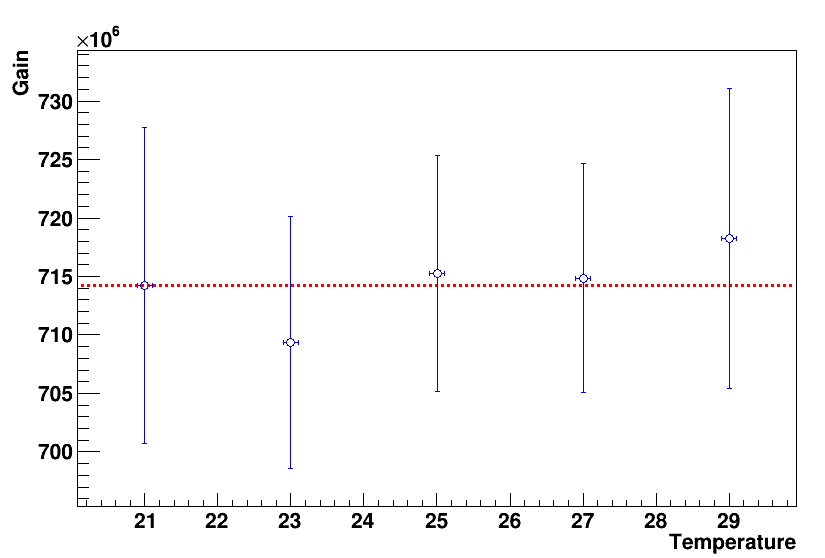
\includegraphics[scale=0.4]{compensacion.png}
\caption{Verificación del método de compensación}
\end{figure}

Donde la raya roja corresponde al ajuste a una constante. Su valor, correspondiente al valor de la ganancia es $G=7.14203 \cdot 10^8 \pm 4.97472 \cdot 10^6$. Comprobamos una última vez la calidad del ajuste a partir del test $\chi^2$ obteniendo un valor de $\frac{\chi^2}{ndf}=\frac{0.318}{4}\approx 0.0795$, valor lijeramente bajo. Este, probablemente, puede ser debido a una sobreestimación de los errores (algo que ya puede apreciarse en la imágen).

Podemos ver que el método funciona de manera muy eficaz ya que la ganancia presenta variaciones muy pequeñas de aproximadamente $\Delta G=5 \cdot 10^6$, que corresponde a una variación relativa de $\sigma_{rel}=2.801 \cdot 10^{-3} $. Hemos comprobado por tanto que se trata de un método realmente eficaz.

La máxima variación se observo a 23 grados. Esta es debido a que fue una medida realizada muchas horas despues de tomarse las otras y existen factores externos que no podemos controlar y afectan al sistema. En este tiempo más largo transcurrido es más probable que hayan cambiado estos factores. Sin embargo puede observarse en todo momento que la variación de la ganancia es mínima verificando en gran medida la ecuación anteriormente obtenida.



\newpage
\section{Prototipos} \label{sec:ch04}
Finalmente, con cada una de las partes convenientemente preparadas y calibradas, procedemos a realizar el estudio sobre una de las configuraciones que contempla el proyecto \textit{Tritium}. Para ello, en primer lugar, se realizará una descripción del prototipo y de la puesta a punto del mismo. En segundo lugar, se presentarán los resultados obtenidos.
	\subsection{Configuración de la electrónica}
	En primer lugar se tuvo que diseñar y construir un prototipo que respondiese a una serie de exigencias impuestas por el experimento. Por un lado este debía de ser capaz de albergar de manera segura  un bunch de 35 fibras centelleadoras, el cual se encontraría totalmente sumergido en una solución de agua tritiada estanca. Este prototipo debía de ser capaz de comunicar los extremos del bunch con contadores de fotones, los cuales deben estar aislados del agua tritiada, sin que existiese ningun tipo de fisura para asegurar que no existe peligro de fuga y, por tanto, de contaminación, nisiquiera por evaporación del agua. Por otro lado debía de sostener de forma segura el contador de fotones utilizado, en nuestro caso PMTs, para leer la señal recibida por estas fibras centelleadoras.

Con todas estas exigencias el materíal elegido para la construcción del prototipo fueron diversos elementos de fontanería de PVC. El motivo de este es su seguridad, ya que están especialmente diseñados para transportar y retener agua, su facilidad de manipulación ya que podemos realizar cortes con mucha rapidez, sencillez y eficacia además de existir muchas formas para diversos fines y, finalmente, su precio ya que se trata de un matería bastante económico. 

En concreto se utilizo un tubo de PVC de 2 metros de longitud y un diámetro interior de 15 mm, en el cual se practicaron una serie de cortes dando lugar a un conjunto de secciones que conformarían los 2 prototipos. Para unir cada una de estas secciones y dar forma al prototipo se utilizaron codos, típicamente utilizados en fontanería de PVC, cuyas uniones serían finalmente selladas con silicona. Finalmente el prototipo quedaría sujeto de forma segura sobre una estructura de metacrilato y acero. El aspecto final del prototipo puede verse reflejado en la figura 20.

\begin{figure}[hbtp]
\centering
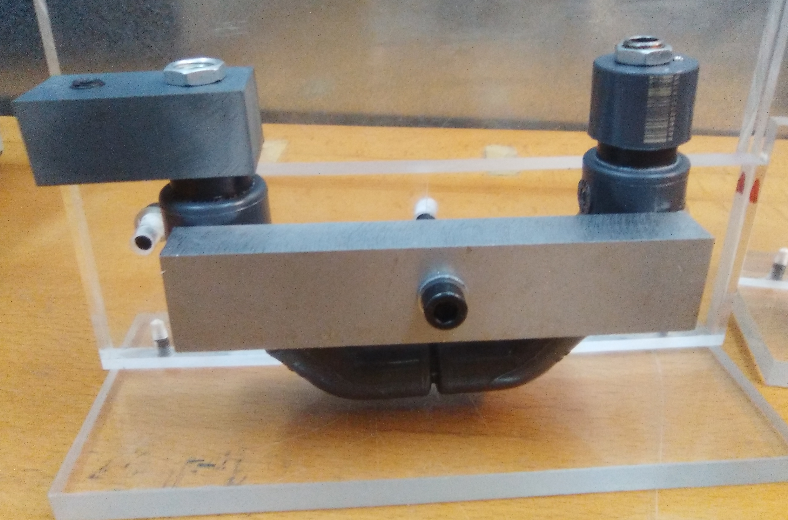
\includegraphics[scale=0.4]{Prototipo.png}
\caption{\textbf{Figura 20}.- Prototipo}
\end{figure}

Este prototipo presenta un volumen en su interior (el cual será rellenado por la soución radiactiva) de $39~\cm^3$, el cual se calculó y verificó con varios ensayos de llenado con agua destilada. También se verificó la permeabilidad del prototipo a partír de una estáncia de estos ensayos de 2 días. 

Podemos observar que se decidió realizar un prototipo con forma de U. Dado que el prototipo no se trasladará en ningun caso y, teniendo en cuenta que se verificó su permeabilidad, personalmente opino que esta es la forma más segura y que mejor se adapta a las exigencias del prototipo. Las dos oberturas superiores serán cerradas y selladas con tapones tipicamente utilizados en fontanería de PVC. Se eligieron tampones diferentes para cada extremo. Un primer tapón circular, acorde a la forma del tubo de PVC y un segundo tapón cuadrado, el cual nos facilitaría el proceso de llenado. Este segundo tapón dispone de dos orificios, uno de 8 mm por el que se realizará el proceso de llenado y otro de 1 mm por el que se purgará el aire durante el mismo proceso. Finalmente estos orificios se cerrarán con ayuda de dos tornillos de rosca envuletos en teflón. Estos tapones pueden verse reflejados en la imagen 20.

Además ambos extremos disponían también de un agujero de 9,8 mm de diámetro, tamaño justo para que por cada uno de estos pasara un extremo del bunch de fibras centelleadoras. En estos extremos se dispusieron dos arandelas, roscadas al aro que conformaba el extremo del bunch, según la imagen 5 (una arandela a cada extremo del tapon, parte interna y externa). De esta forma conseguíamos fijar perfectamente cada uno de los extremos del bunch al prototipo y comunicar el extremo de las fibras al exterior del prototipo para su correspondiente lectura con los contadores de fotones, PMTs en nuestro caso. 

En todo momento se utilizó silicona para sellar cualquier posible fisura del prototipo.

También podemos observar que se ha decidido realizar el giro de $180º$, correspondiente a la U, con ayuda de cuatro codos de $45º$ y no con dos codos de $90º$. Esto es debido a que, con giros progresivos, el bunch de fibras centelleadoras estarán sometidos a una tensión inferior y, por extensión, ofrecerán una mejor propagación de la señal.

Finalmente se utilizaron dos piezas, usualmente utilizadas en fontanería de PVC para comunicar tuberías de igual o diferente diámetro para sostener los PMTs en el prototipo. Debido al hecho de haber utilizado dos tapones distintos ahora necesitaremos dos piezas diferentes. Estas pueden verse en la figura veinti uno.

\begin{figure}[hbtp]
\centering
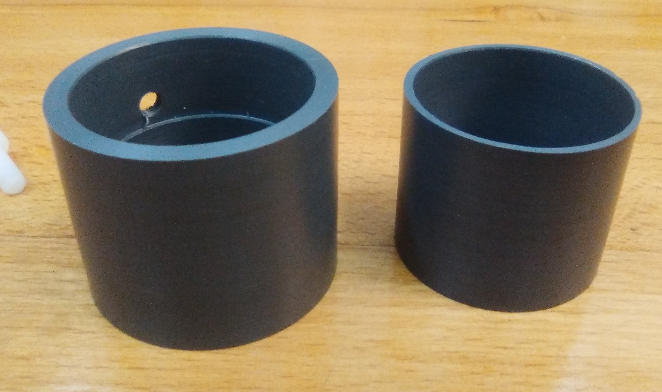
\includegraphics[scale=0.4]{Tapones.png}
\caption{\textbf{Figura 21}.- Piezas de sujeción de los PMTs}
\end{figure}

La primera pieza (correspondiente a la pieza derecha de esta figura), más pequeña, simplemente encajaba al tapón circular por un extremo y, por el otro, con un diámetro interior más grande para que cupiese y fijase, se disponía del PMT.

Para la segunda pieza encontramos un problema y es que no hay tuberías cuadradas, por lo que no encontramos ningun tipo de pieza como esta que ajustase a este tapón (tapón cuadrado del prototipo). En su lugar simplemente utilizamos una pieza para que encajase a la arandela que sobresalía del prototipo (utilizada para fijar el bunch de fibras) y por el otro extremo que encajase al PMT. Para mayor sujeción se utilizo en esta pieza un tornillo que unía esta a la plataforma de metacrilato. La disposición de estos en el prototipo y el tornillo que ayuda a la sujeción pueden verse reflejados en las imágenes de la figura veinti dos.

\begin{figure}[htb]
\centering
{
%\subfloat[Espectro de emisión]
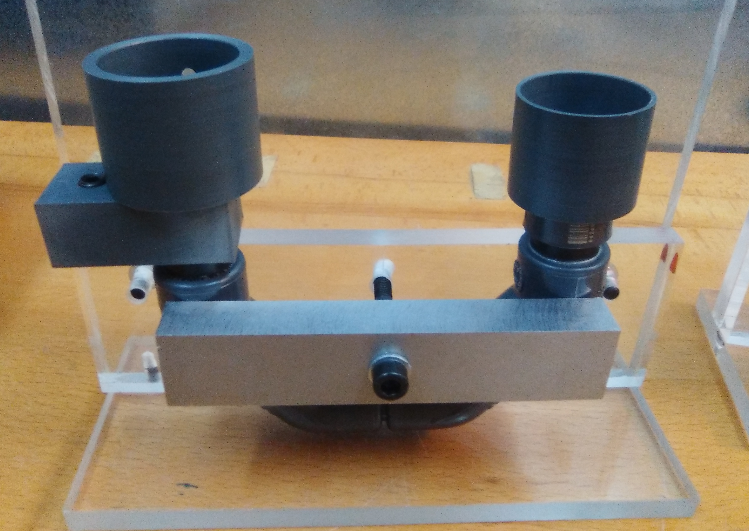
\includegraphics[scale=0.25]{Prototipodelantetapon.png} 
}
{
%\subfloat[Espectro de emisión]
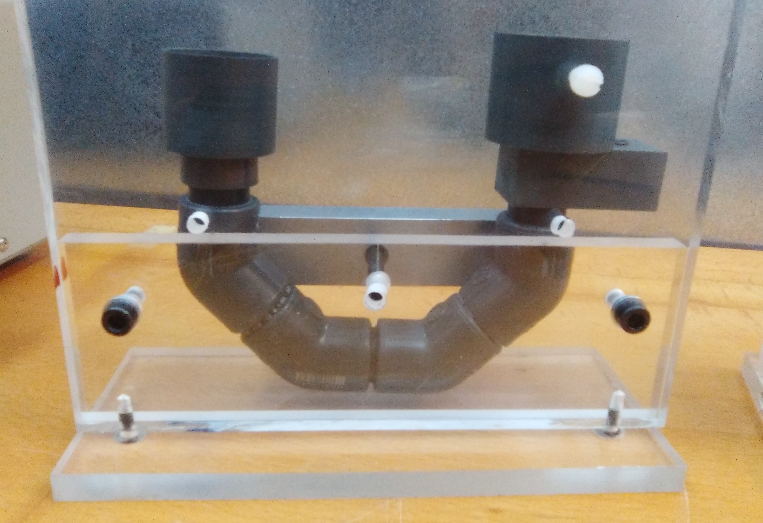
\includegraphics[scale=0.25]{PrototipoDetrastapon.png} 
}
\caption{\textbf{Figura 21}.-Cara fibras}
\end{figure} 

Hay que tener en cuenta que el proceso de medida se desarrollará en el interior de una cámara oscura cuya única labor es la de protejer de la posible entrada de luz del exterior. En esta no habrá un control exhaustivo de la temperatura como ocurría con el sistema utilizado para la calibración de los SiPM. En su lugar únicamente activaremos el aire acondicionado en la sala para mantener una temperatura constante de aproximadamente $25ºC$ en todo momento.

Los PMTs empleados, R8520-ZB2771 y R8520-ZB2773 se alimentaron ambos a $-830$ V. A esta temperatura disponen de una ganancias de $G_1=1456178$ y $G_2=1921595$ y su eficiencia de fotodetección a $\lambda=430nm$ es de $29.76\%$ y $28.66\%$ respectivamente. 

	
	\subsection{Procedimiento de llenado}
	Para realizar el llenado en primer lugar necesitamos preparar la solución de agua tritiada. Para ello disponemos de una fuente radiactiva de tritio, es decir, una solución de agua tritiada ($HTO$ en $\ce{H_2}O$) de $2.0169 \pm 0.0017\gram$ de peso y una actividad específica de $A=26.8 \pm 0.6~\mega\becquerel/\gram$ con fecha de calibración del 16 de marzo de 2017. Esta fuente presenta una actividad tal que puede considerarse exenta~\cite{IFIC}
.

Esta ha sido proporcionada por PTB (Physikalisch-Technische Bundesanstalt, Braunscheweig and Berlin), Alemania. Presenta un número de serie 2005-1442, un número de referencía PTB-6.11-285/03.2017, una fecha de referencia de 1 de enero de 2017~\cite{IFIC}
.

La solución que prepararemos para el experimento, denominada solución patrón, consiste en diluir la ampolla que contiene la solución anterior con 0.5L de agua hiperpura, la cual ha sido proporcionada por el LAREUX de Cáceres, Universidad de Extremadura. Esta disolución fué realizada por Teresa Cámara en el laboratorio de radiactividad ambiental, LARAM, de la universidad de Valencia.

El agua hiperpura consiste...

Finalmente, con la solución patrón ya preparada, se realizó el proceso de llenado en la gammateca del IFIC, sala debídamente acondicionada para manipulacón de fuentes radiactivas. Se prepararon un total de $50~\cm^3$ de solución patrón.

El mecanismo seguido para el proceso de llenado se describe a continuación:

\begin{enumerate}
\item{} En primer lugar se dispuso de una bandeja de plastico recubierta con material absorbente en el interior de la cual se realizaría todo el proceso de llenado. El objetivo de esta fue evitar en la medida de lo posible una contaminación debido a un desbordamiento en el proceso de llenado. 

\item{} En segundo lugar, con ayuda de una pipeta y un embudo de crital, se procede a llenar una bureta. Para mayor seguridad se fijo la bureta con un soporte de laboratorio. 

\item{} En tercer lugar, con la bureta ya llena del agua tritiada, se procede a introducir esta en el prototipo. Para ello se introduce la punta final de la bureta en el orificio de 8 mm del prototipo anteriormente descrito y, lentamente, se procede al llenado del mismo. El proceso terminará en el momento en que se hayan introducido $39~\cm^3$ ya que, como se ha mencionado anteriormente, este es el límite del prototipo.

\item{} En cuarto lugar se procederá a cerrar los dos orificios del prototipo anteriormente mencionados. Además, el resto de la disolución sobrante se verterá en una botella suficientemente segura en la cual se conservará para un futuro uso. Esta disolución junto con el material empleado en el proceso de llenado se introducirá en una bolsa de plastico, la cual se introducirá en una caja de carton, y todo ello será debidamente guardado en el LARAM.

\item{} En último lugar se trasladará el prototipo, debidamente rellenado y sellado, al laboratorio de reaciones nucleares del IFIC (025)

\end{enumerate}


	
	\subsection{Configuración de la electrónica}
	Finalmente, con cada una de las partes del prototipo debidamente conectadas y calibradas y la fuente de tritio debidamente situada y asegudara, únicamente nos resta configurar la parte electŕonica del sistema para empezar a medir en el prototipo y obtener una señal adecuada. El objetivo será obtener un espectro energético de experimento con ayuda de un analizador multicanal analógico, MCA con tarjeta PCA3 y un programa Oxford WIN-MCA. 

Para ello necesitamos realizar una seríe de transformaciónes a la señal para que, por un lado,  pueda ser analizada de manera adecuada por el MCA y, por otro lado, optimicemos al máximo la señal sobre el background. El esquema electrónico utilizado se muestra en la figura veinti dos.

\begin{figure}[hbtp]
\centering
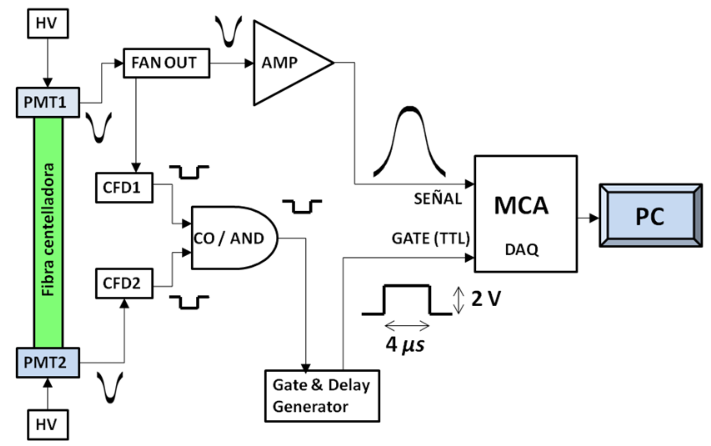
\includegraphics[scale=0.4]{Esquemaelectronico.png}
\caption{\textbf{Figura 22}.- Esquema Electrico~\cite{Andres}}
\end{figure}

Para conseguir cada uno de estos pasos se ha utilizado tecnología NIM. A continuación se procede a explicar el camino seguido por la señal y cada uno de los módulos que intervienen en estas transformaciones:

\begin{enumerate} 
\item{} En primer lugar sacaremos la señal de cada fotomultiplicador de la caja negra utilizada para apantallar la luz del exterior. Ello lo conseguimos con ayuda de cables BNC  ya que la caja dispone de puertos BNC macho que comunican el interior y el exterior.

\item {} Seguidamente dividimos la señales de un PMT en dos señales idénticas con ayuda de un divisor activo FAN IN/FAN OUT. Esta no es una simple división de la señal donde se produce un reparto de la intensidad sino una copia exacta de la señal de entrada. Necesitamos este típo de módulo y no una simple división ya que, como se explico al inicio del trabajo, la señal de tritio es una señal muy debil por lo que no nos podemos permitir tener pérdidas ni divisiones de esta.

\item {} Ahora dividiremos en dos caminos. Por un lado una copia de la señal del PMT que se ha duplicado, se llevará a un preamplificador (marca Tennelec) y, seguidamente, a un amplificador (marca Tennelec, modelo TC 241) con una ganancia configurada de 50. Con este camino conseguimos amplificar de manera adecuada la señal de un PMT, del orden de 60 mV hasta un total de 3V, lo cual nos permitirá optimizar el rango disponible en el MCA (Entre 0 y 5 V). Nos referiremos a la señal obtenida por este camino como señal 1.

\item{} Por otro lado, las dos señales restantes (una señal de cada PMT) serán llevada por un camino distinto para obtener una señal que nos indique cuando hay coincidencia. Para conseguir esta segunda señal hay que tener en cuenta que los PMTs ofrecen señales analógicas y negativas. Por tanto, dado que esta señal de coincidencia será creada y tratada con tecnología NIM, necesitamos convertir estas señales en señales lógicas de estándar NIM. 

Esto lo conseguimos pasando cada una de estas dos señales por un módulo discriminador (CAEN, de cuatro canales). Este ofrece una señal lógica en forma de escalón negativo de altura 1 voltio y anchura variable, en nuestro caso $30~\ns$, para cada una de las señales siempre y cuando la señal de entrada asociada supere un umbral determinado, en nuestro caso 30 mV (hablamos en valores absolutos, hay que tener en cuenta que estas son negativas). De esta forma eliminamos de manera considerable el dark current de los PMT y, por extensión, el background.

\item{} A continuación hacemos pasar ambas señales de la salida del discriminador por un módulo de conicidencias modelos Cern N 6234. Este genera una señal de salida si solo si las dos señales de entrada (procedentes de cada PMT tras pasar por el discriminador) están en coincidencia temporal. 

Estas cuatro señales (PMT, puerta lógica de cada PMT y puerta lógica de coincidencia) pueden verse en la siguiente figura:

\begin{figure}[hbtp]
\centering
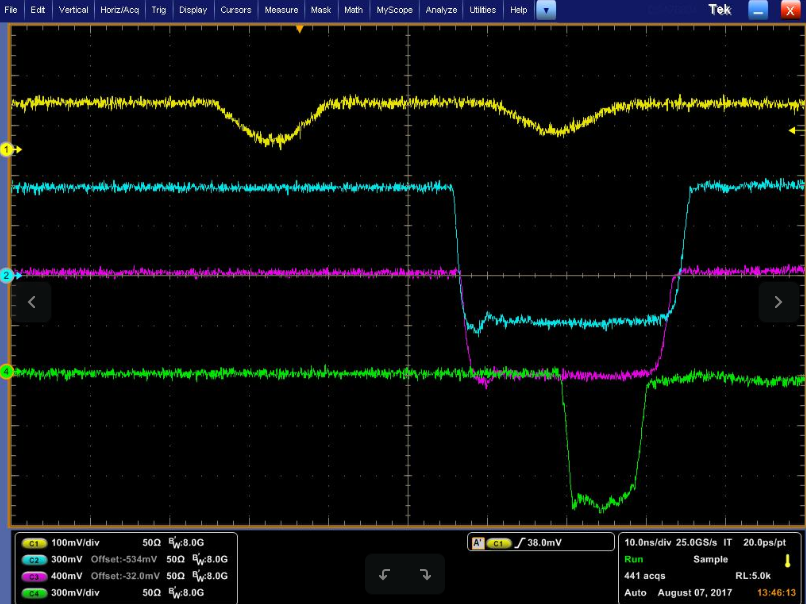
\includegraphics[scale=0.4]{SenalesNIM.png}
\caption{\textbf{Figura 24} Señal de salida del PMT (1), señal de salida del discriminador para cada PMT (2 y 3) y señal de salida del módulo de concidencias respectivamente}
\end{figure}


\item {} Luego pasamos esta señal de coincidencia a un módulo Gate \& Delay Generator (marca ORTEC, modelo 416A). Este módulo nos genera una señal lógica en forma de escalón positivo, de altura 2 voltios y anchura de $4~\mu s$, anchura suficiente para comprender en su interior la totalidad de la señal 1. Esta puerta debe ser positiva debido a que este es un requisito del MCA. Además aplicaremos un retraso a esta señal que compense la diferencia de caminos seguidos entre esta y la señal 1. Nos referiremos a la señal obtenida por este camino como señal 2.

\item {} En último lugar pasarmemos al MCA tanto la señal 1 (señal de un PMT amplificada) como la señal 2 (que nos indica cuando ambos fotomultiplicadores han detectado en coincidencia). Estas dos señales pueden verse en la siguiente figura.

\begin{figure}[hbtp]
\centering
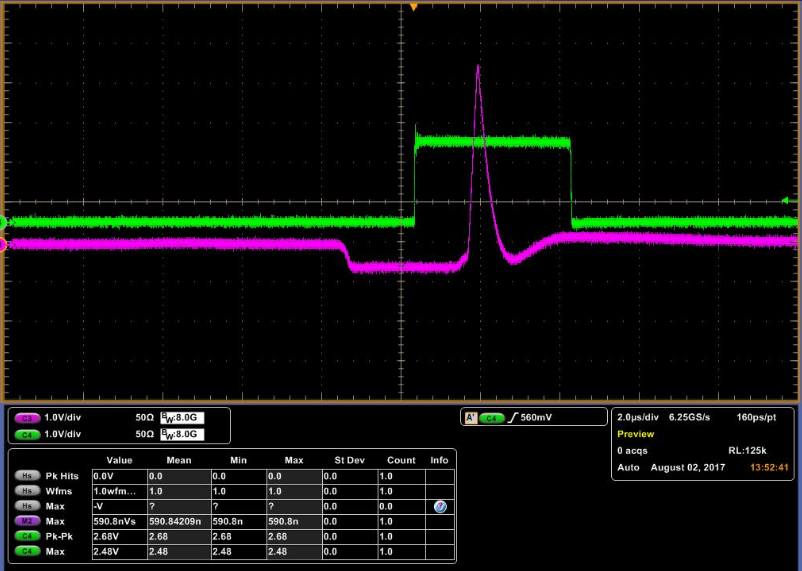
\includegraphics[scale=0.4]{SenalesMCA.png}
\caption{\textbf{Figura 24} Señales de entrada del MCA}
\end{figure}


Este MCA dispone de la opción de crear un histograma de señal 1 la cual solo leera mientras la señal 2 sea no nula, es decir, solo leera la señal 1 en la ventana proporcionada por la señal 2. Aquí reside la importancia de ajustar bien la anchura de la señal 2 ya que, debe de ser suficiente para contener en todo momento la señal 1 pero ajustada tanto como sea posible para evitar la entrada de dark current.

Con esto conseguimos realizar una detección en coincidencia de ambos fotomultiplicadores, lo cual nos reducirá enormemente el background del experimento.

\end{enumerate}




	
	\subsection{Resultados}
	Ahora, dado que ya disponemos de todas las partes del sistema convenientemente dispuestas y calibradas, procedemos a realizar una primera medida.

Hay que tener en cuenta que en estas primeras medidas no necesitamos un sistema de control de temperatura ya que vamos a utilizar PMT y estos no son tan sensibles a la temperatura como los SiPM. Únicamente deberemos ser capaces de evitar oscilaciones grandes de temperatura ($\Delta T=15-20ºC$), los cuales si afectan de forma apreciable a la ganancia del PMT. Esto lo podemos conseguir manteniendo el aire acondicionado de la sala experimental encendido y programado a una misma temperatura durante las medidas. 

Sin embargo, cuando vayamos a realizar las medidas del prototipo con SiPMs, si necesitaremos este control exaustivo de la temperatura ya que, como se vió en la sección de calibrado del SiPM, \ref{sec:Temperatura}, existe una dependencia muy marcada. Se necesitará adquirir un sistema de control de temperatura o, en su defecto, como construir y calibrar uno nosotros mismos.

La primera medida se realizará sin coincidencia, pasando directamente la señal 1 al MCA. El MCA nos permite obtener un histograma energético.

Se obtendrá un primer histograma del prototipo con agua hiperpura y sin tritio. Dado que el agua hiperpura idealmente no añade ningun tipo de contribución al histograma llamaremos a esta medida señal de fondo. 

Seguidamente se rellenará el prototipo con agua tritiada y se obtendrá un segundo histograma. En esta segunda medida se pude observar en el display del MCA que el número de cuentas medidas por segundo era mayor que el la medida del fondo. Esto es un indicativo de que estamos detectando tritio. 

Finalmente se normalizan cada uno de los histogramas al tiempo correspondiente a su medida para obtener histogramas de actividad en lugar de un histograma de sucesos. Los tiempos asociados al histograma del tritio y del fondo son $T_S=154143~\second$  y $T_B=246987~\second$, respectivamente, medidas largas para tener suficiente estadística. El resultado puede verse en la figura 26 izquierda. Además se ha añadido una segunda imagen, figura 26 derecha, en la cual se ha realizado representado la señal con tritio a la cual se le ha extraido la señal de fondo, es decir, en esta segunda imagen encontramos la señal debida únicamente al tritio.

\begin{figure}[hbtp]
\centering
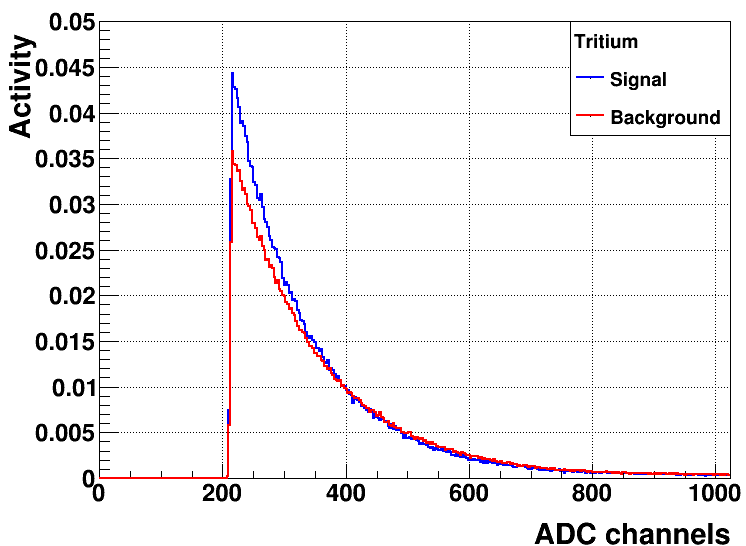
\includegraphics[scale=0.4]{Tritium3-fcpst2.png}
\caption{Histograma energético de la señal del prototipo de tritios y del fondo superpuestos.\label{tritiofondo}}
\end{figure}

En esta figura podemos observar que estamos detectando un pico de señal de aproximadamente $0.045~\becquerel$ y una señal debida únicamente a tritio de aproximadamente $0.01~\becquerel$. POdemos apreciar la existencia de una zona entre los canales 450 y 700 donde el fondo supera a la señal. Habrá que indagar más en este prototipo para encontrar la explicación de este fenómeno.

Para ver hasta que punto nuestro sistema funciona de forma adecuada podemos realizar un rápido cálculo para ver cual es la actividad detectada que deberíamos esperar. Para ello por un lado calcularemos el volumen efectivo de la fuente y, por otro lado, utilizaremos este volumen para determinar cual es la actividad que deberíamos medir teóricamente en nuestro experimento.

\begin{itemize}
 \item{} Para calcular el volumen efectivo de la fuente tenemos en cuenta que los electrones procedentes de la desintegración del tritio poseen un recorrido libre medio de $5~\mu m$. Por tanto únicamente contribuira de forma apreciable a la señal el agua tritiada que se encuentre formando un cilindro de groson $5~\mu m$ alrededor de cada fibra. Pasamos a calcular este volumen. Para ello calcularemos el volumen total y, a esta cantidad, le extraeremos el volumen ocupado por la fibra.

El volumen de la fibrá es el volumen correspondiente a un cilindro de radio $0.5~\mm$ (radio de la fibra) y una longitud efectiva de $20~\cm$, donde se ha tenido en cuenta que, aunque la longitud real de la fibra son $25~\cm$, esta contiene en los extremos del bunch unos aros metálicos y, además, parte de esta fibra sobresale del prototipo para acoplar a los PMTs. Por extensión, esta sección de la fibra, aproximadamente $2,5~\cm$ a cada extremo,  no contribuyen a la señal de detección del tritio. Con todo esto el volumen ocupado por la fibra será $V_{fibra}=1.5708 \cdotp 10^{-4}$ litros.

Análogamente calculamos el volumen ocupado por la fuente más la fibra, que corresponderá a un cilindro de radio $0.5~\mm+5\mu m$ (radio de la fibra + radio efectivo de la fuente) y la misma longitud que la fibra, es decir, $20~\cm$, ya que en estos extremos se encuentra el final del prototipo. Como resultado el volumen ocupado por la fibra y la parte de la fuente que contribuye a la señal de esta fibrá será $V_{total}=1.6023 \cdotp 10^{-4}$ litros. 

Por tanto el volumen ocupado únicamente por el porcentaje de la fuente que esta interviniendo en la señal de esta fibra será la diferencia entre estos $\V_{fuente}=3.1573 \cdotp 10^{-6}$ litros.
 
Por tanto, teniendo en cuenta que el prototipo únicamente dispone de un bunch formado por 35 fibras centelleadoras el volumen efectivo final del agua tritiado que estamos detectando será el anterior multiplicado por 35, es decir, $1.1050 \cdotp 10^{-4}$ L. 

Hay que tener en cuenta que en esta última multiplicación se ha supuesto que el volumen del agua tritiada asociadas a cada fibra forman un conjunto disjunto y sabemos que esto no es así ya que se producen solapamientos entre ellos. Debido a ello este cálculo será únicamente aproximado.

\item{} Ahora procedemos a calcular la actividad del prototipo conociendo el volumen de agua tritiada que esta aportando a la señal total. Para ello tenemos en cuenta que la disolución posee $2.0169 \pm 0.0017~\gram$ de tritio con una actividad específica de $26.8 \pm 0.6~\mega\becquerel/\gram$ disueltos en medio litro de agua hiperpura (Sec. $\ref{sec:Llenado}$). Con esto podemos calclularnos la actividad total de la disolución, la cual será aproximadamente de $108.11~\mega\becquerel/L$. 

Por tanto, si en medio litro hay aproximadamente $1.0811\cdotp 10^{8}$ desintegraciones por segundo en el volumen calculado anteriormente habrá aproximadamente $2.3893\cdotp 10^{4}$ desintegraciones por segundo.

Finalmente, teniendo en cuenta que la eficiencia de la fibras y de los PMTs son, aproximadamente, 3\% y 30\% respectivamente y suponiendo que la cadena electrónica posee una eficiencia del 100\% llegamos a que la actividad que deberíamos detectar es, aproximadamente $215.03~\becquerel$.

\end{itemize}

Podemos ver que estamos detectando 4 ordenes de magnitud menos de lo que deberíamos. Por un lado esto es debido a imperfecciones del sistema pero la principal fuente de la pérdida de la señal es el hecho de que las fibras empleadas en este prototipo no poseen clad. 

El clad hace que los fotones sean conducidos por el interior de las fibras a partir de reflexiones hasta el contador de fotones, es decir, actua como guia de luz, por tanto, en nuestro prototipo, muchos de los fotones de emisión de las fibras escaparán de estas llegando al agua y, por tanto, producirán pérdida de señal. 

Como resultado únicamente detectaremos el porcentaje asociado al ángulo sólido cubierto por las fibras centelleadoras respecto al total de electrones emitidos por el tritio, cuya emisión supondremos isótropa. Además, del total de fotones reemitidos por las fibras centelleadoras (de nuevo se supone emisión isótropa) ante la detección de este electrón, únicamente detectaremos el porcentaje asociado al ángulo sólido cubierto por la cara final de la fibra centelleadora. También hay que tener en cuenta que el porcentaje de fibra que se encuentra en la parte inferior de la U que conforma el prototipo apenas intervendrá en la señal ya que vemos que prácticamente la totalidad de esta será perdida (su ángulo sólido es cero). 

Podemos realizar una rápida estimación de la magnitud relativa de estos ángulos sólidos para ver su importancia en la pérdida de la señal. Integrando la expresión del ángulo sólido esta toma la siguiente forma: $\Omega=2\pi(1-\cos{\theta})$ donde $\theta$ es el ángulo que subtiene la superficie que queremos calcular$~\cite{unizar}$. Por tanto, dado que la superficie total de emisión será $4\pi$ ($\theta=180º$) el factor de reducción debido al ángulo sólido será $\frac{\Omega}{4\pi}=\frac{1-\cos{\theta}}{2}$. 

Si nos calculamos el ángulo y, por extensión, este factor para el caso del ángulo sólido subtendido por la fibra centelleadora vemos que este ángulo siempre será aproximadamente $90º$ debido al hecho quela fibra centelleadora es mucho mayor que su destancia punto de la desintegración, $5\mu m$ como máximo. Por tanto este factor será aproximadamente $0.5$ en todo momento, es decir, aproximadamente la mitad de los electrones que se producen en este punto del agua tritiada pasan por la fibra. Sin embargo, la reemisión de fotones de las fibras al detectar un electrón posee un factor realmente pequeño. Por ejemplo, un punto situado a 2 cm de la cara final de la fibra posee un factor de $3.12\cdotp 10^{-4}$ llegando a valer $0$ para los puntos correspondientes a la parte inferior del prototipo como se ha mencionado anteriormente. Vemos por tanto que si llega a ser un factor realmente relevante y que podría explicar esta gran pérdida de señal. 

Por tanto, debida a la necesidad de recolectar el máximo de luz, un paso inmediato en el siguiente prototipo será incluir fibras con clad que nos permitan recolectar un mayor porcentaje de luz. El problema reside en que el grosor actual del single clad comercial de las fibras Saint-Gobain es de, aproximadamente, $4\%$ del diametro, es decir, $40~\mu m$. Prácticamente ningun electrón conseguirá pasar el clad y ser detectado en el núcleo de la fibra por lo que habrá que considerar otros mecanismos de guia de ondas. Una posible solución a este problema sería incluir nosotros el clad en las fibras a partir del proceso de vaporación de aluminio por evaporación en vacío. Esto lo podemos realizar en el ICMOL, departamento asociado al IFIC, con el cual ya se han realizado trabajos similares anteriores. De esta forma podríamos conseguir un clad con un espesor del orden de cientos de nanometros, espesor suficientemente pequeño para que un porcentaje aceptable de electrones derivados de la desintegración del tritio puedan superarlo. 

\newpage
\section{Simulaciones} \label{sec:ch04}
Finalmente presentamos en este último punto las simulaciones realizadas sobre el experimento. Estas han sido desarrolladas sobre un codigo bastante avanzado sobre el que se han realizado una serie de modificaciones. Pretenden simular un prototipo del detector rectilineo a diferencia del nuestro que presenta forma de U. Una imagen transversar del prototipo puede verse reflejado en la figura 27.

\begin{figure}[hbtp]
\centering
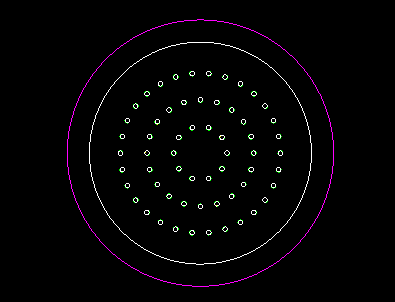
\includegraphics[scale=0.4]{Finalforntal.png}
\caption{Imagen transversal del prototipo\label{imagenprototiposimulado}}
\end{figure}


Está formado por un cilindro externo de teflon  de radio interno $2.5~\cm$, medio centimetro de grosor y una longitud de $80~\cm$ dando lugar a un volumen interno de $1.1781~l$. En su interior residirán 60 fibras centelleaoras dispuestas formando 3 círculos segun la imagen 27. El círculo interno, con un diámetro de $6~\mm$, contendrá 10 fibras, el círculo intermedio, con un diámetro de $12~\mm$, contendrá 20 fibras y el círculo externo, con un diámetro de $18~\mm$ contendrá 30 fibras. El volumen efectivo interno (descontando el volumen ocupado por las fibras) será de $1.1498~l$, volumen que en la práctica será ocupado por el agua tritiada.

Las fibras que se han simulado pretenden ser las utilizadas hasta el momento, fibras centelleadoras BCF-12 de un milimetro de diámetro pero con longitud de 60 centímetros. En los 20 centímetros del cilindro de teflon que no están ocupados por las fibras centelleadoras (10 cm a cada lado) se pretende situar los PMTs o, en su defecto, los SiPMs para detectar los fotones que reciban de las fibras. Ambos lados estarán separados por una ventana de quarzo que permita el paso de los fotones y no del agua destilada ya que ninguno de los contadores de fotones que utilizarán en este experimento puede encontrarse en contacto con el agua en ningun momento.

La simulación describe la emisión de una fuente de tritio que en la práctica se encontrará cubriendo por completo el volumen libre del interior del cilindro de teflon pero, con el objetivo de agilizar las simulaciones, solo ha sido necesario implementar un interior de aire y unos cilindros de agua tritiada de $50~\mu m$ de grosor alrededor de cada fibra centelleadora. Debido a que el recorrido libre medio de los electrones en el agua es $5~\mu m$ ambas situaciones son análogas. 

Hay que tener en cuenta que los resultados presentados de estas simulaciones únicamente describen los electrones detectados en las fibras y la posterior conversión de estos en fotones. En esta simulación no se ha implementado el posterior tratamiento de la luz, por lo que todavía no podemos justificar la importancia de la pérdida de luz discutida en la seccion $\ref{sec:Resultados}$

Los resultados obtenidos para una simulación de 10000 eventos se muestran a continuación:
\begin{enumerate}
\item{} En primer lugar se ha realizado un histograma energético de los electrones emitidos en la desintegración del tritio, el cual se muestra en la imagen 28.

\begin{figure}[hbtp]
\centering
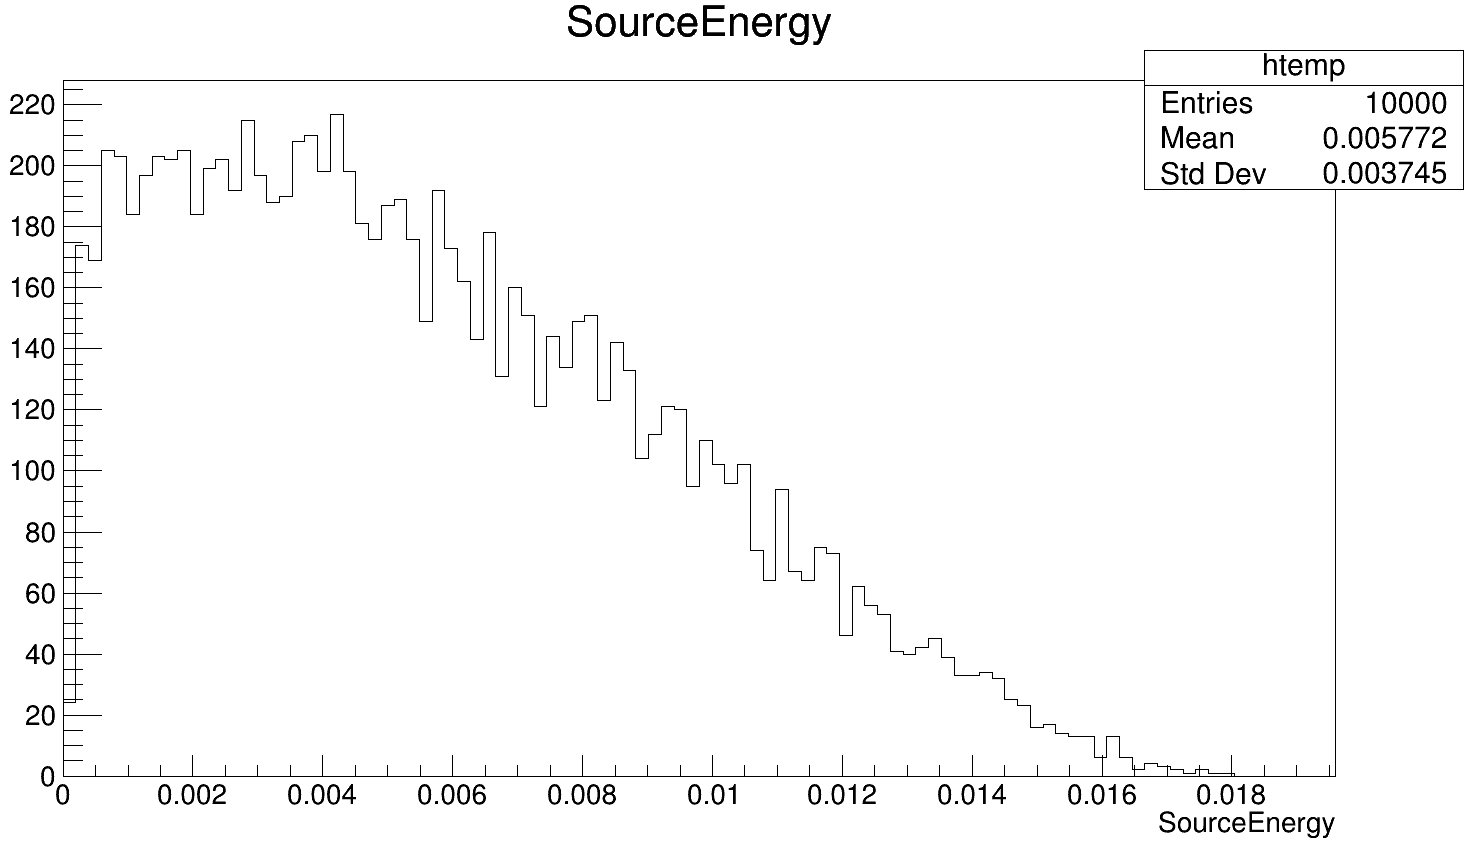
\includegraphics[scale=0.2]{espectrotritiosimulado.png}
\caption{Espectro simulado de los electrones procedentes de la desintegración del tritio (Escala en MeV)\label{espectrotritiosimulado}}
\end{figure}

Podemos ver que se trata de un espectro que se ajusta perfectamente al espectro teórico, fig. $\ref{Espectrotritio}$. Para conseguir un espectro más suave será necesario realizar una simulación con un mayor número de eventos, para lo cual será necesario acceder al centro de cálculo del IFIC para disponer de de una mayor potencia de computación.

\item{} Seguidamente se realizo un histograma de la posición de la fibra en la cual se había detectado el suceso. Este se muestra en la siguiente figura en la que se muestran tres imágenes asociadas a cada uno de los ejes espaciales.

\begin{figure}[htb]
\centering
{
%\subfloat[Espectro de emisión]
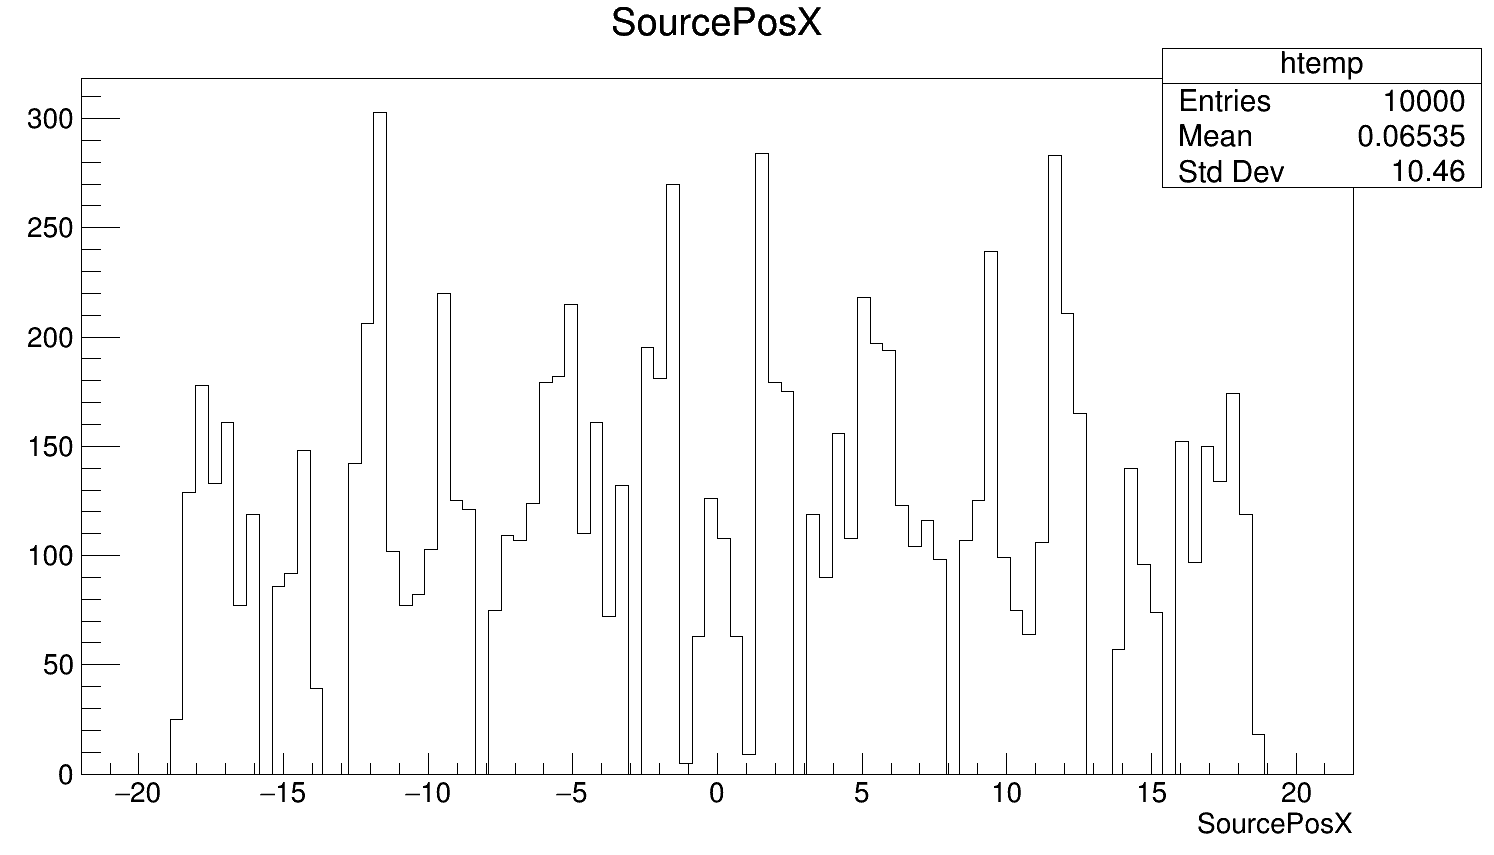
\includegraphics[scale=0.1]{eventosXfibras.png} 
}
{
%\subfloat[Espectro de emisión]
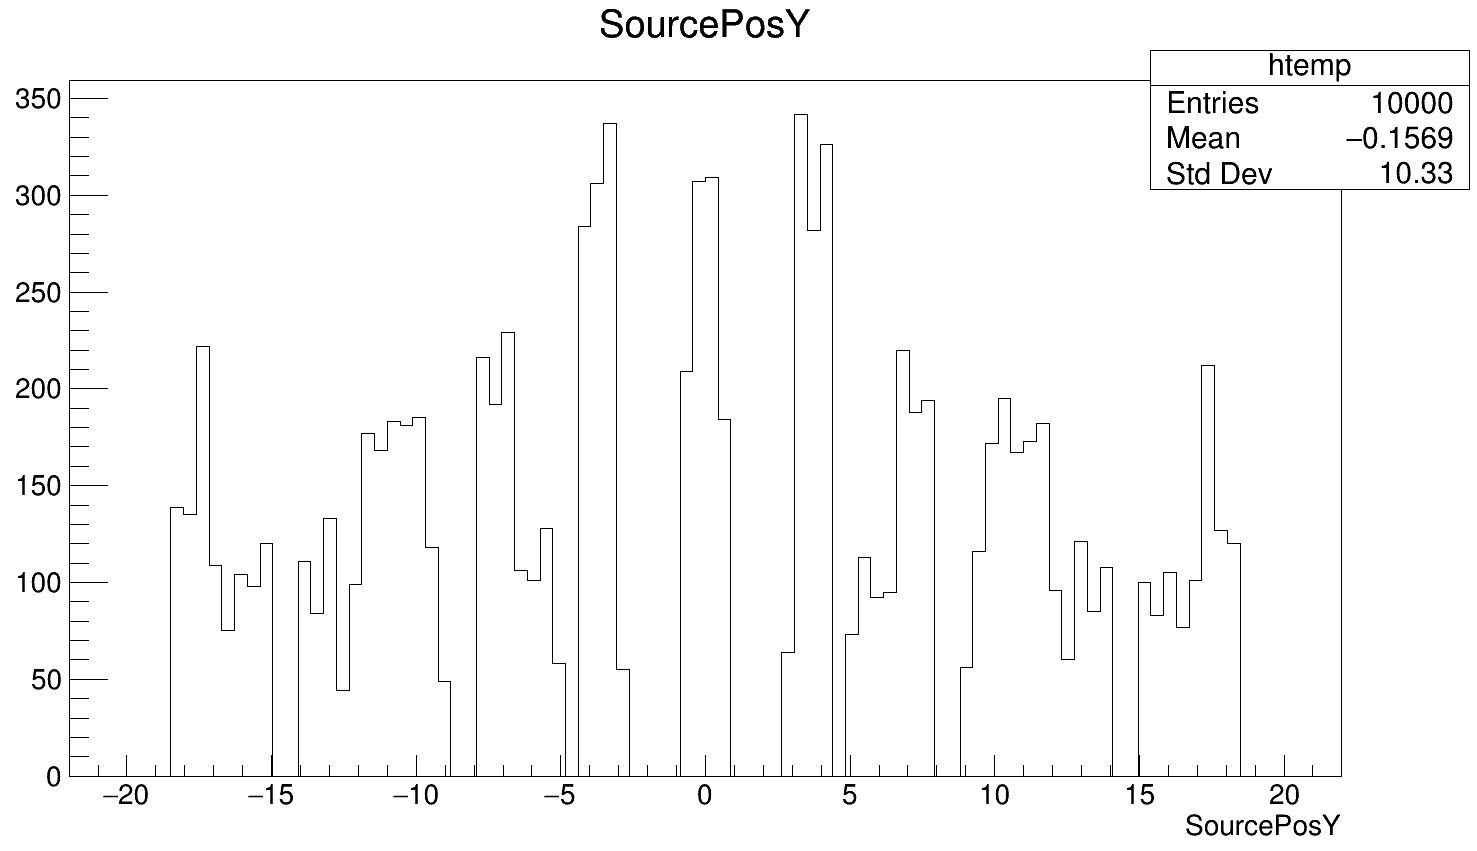
\includegraphics[scale=0.1]{eventosYfibras.png} 
}
{
%\subfloat[Espectro de emisión]
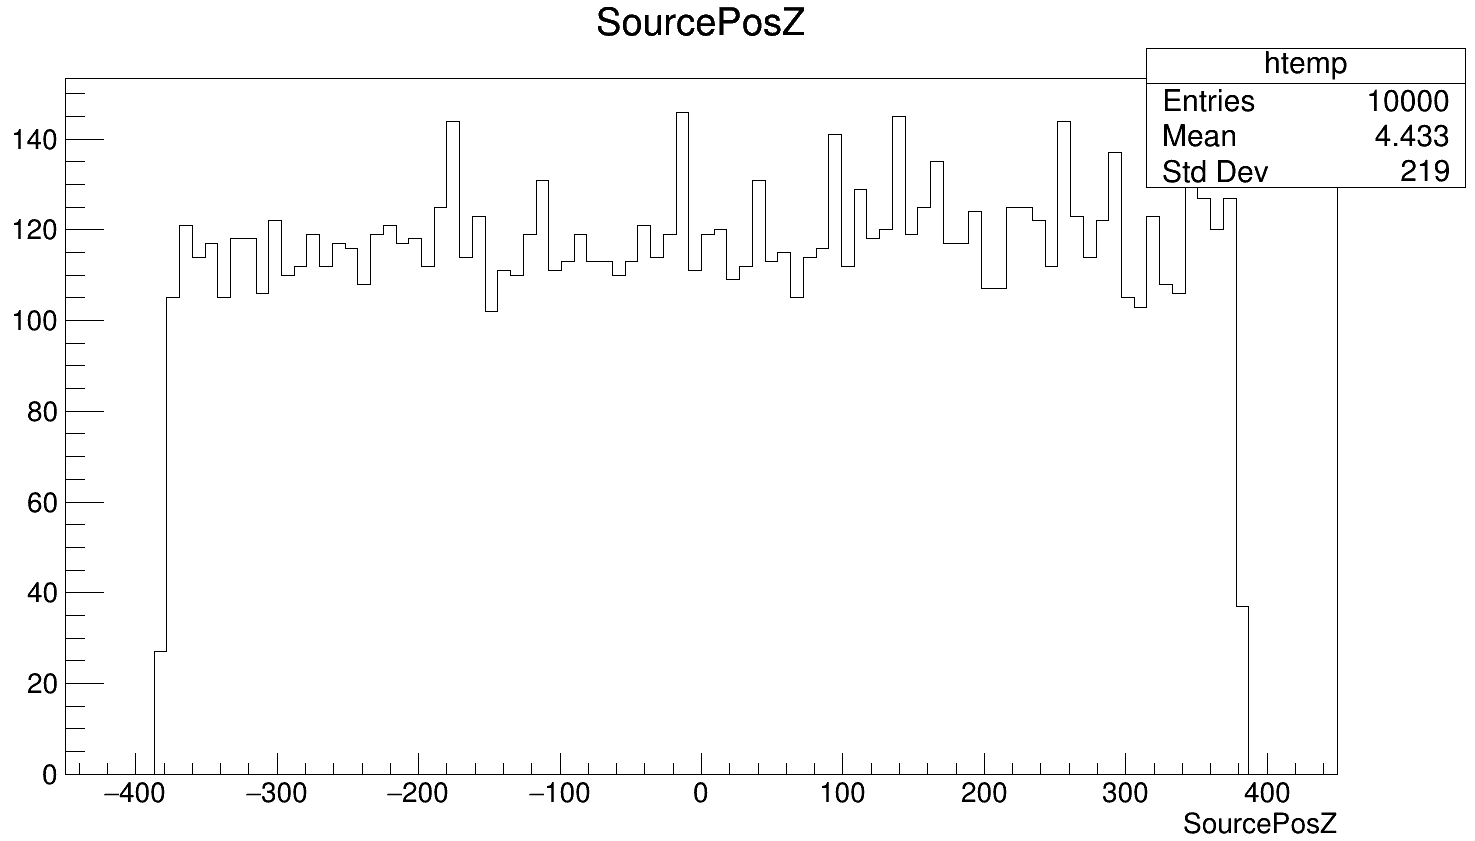
\includegraphics[scale=0.1]{eventosZfibras.png} 
}
\caption{Histograma espacial de la posición de detección de los electrones en las fibras\label{espectroespacial}}
\end{figure}

En los ejes X e Y puede apreciarse una detección más o menos uniforme en los puntos espaciales donde se encuentran situadas las fibras y, en el eje Z puede apreciarse una detección totalmente uniforme a lo largo de la longitud de las fibras. Este es un resultado que deberíamos esperar ya que se ha simulado una fuente de actividad uniforme y constante en el tiempo.

\item{} Se ha asignado un número del 1 al 60 a cada una de las fibras y se ha realizado un histograma del número de eventos que se han detectado en cada una de ellas. Este se muestra en la figura 30.

\begin{figure}[hbtp]
\centering
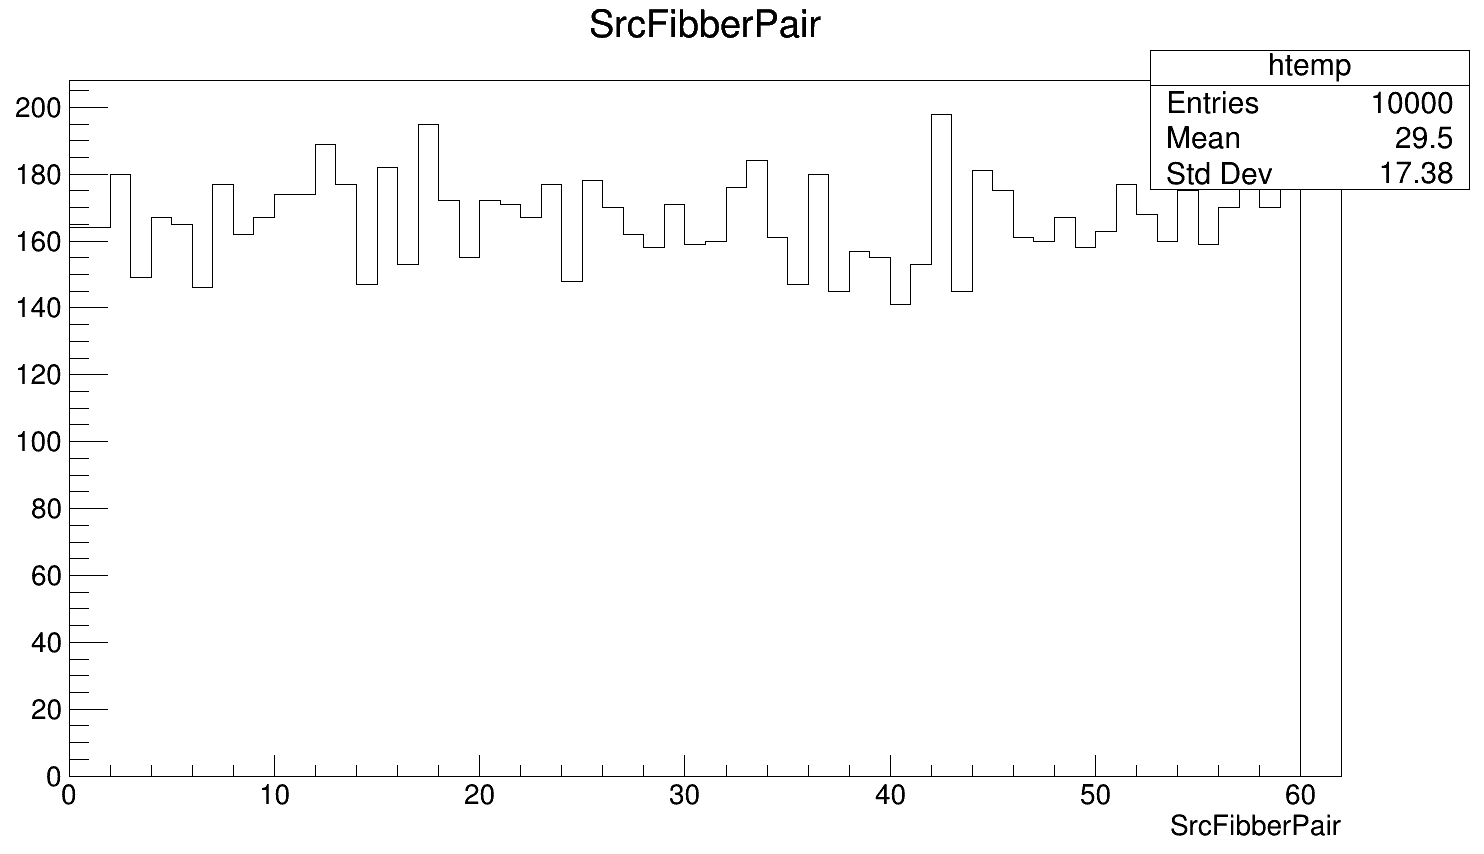
\includegraphics[scale=0.2]{Histogramafibras.png}
\caption{Histograma de sucesos sobre cada fibra\label{sucesossobrecadafibra}}
\end{figure}

Podemos observar de nuevo que se trata de una deposición uniforme sobre las fibras. Todas han detectado aproximadamente el mismo numero de eventos, algo que de nuevo deberíamos esperar.

\item{} Seguidamente se ha obtenido el espectro de energía depositada en el agua y en las fibras además de las longitudes recorridas en ambos medios por los electrones del tritio. Ambas se muestran en las figuras 31 y 32 respectivamente

\begin{figure}[htb]
\centering
{
%\subfloat[Espectro de emisión]
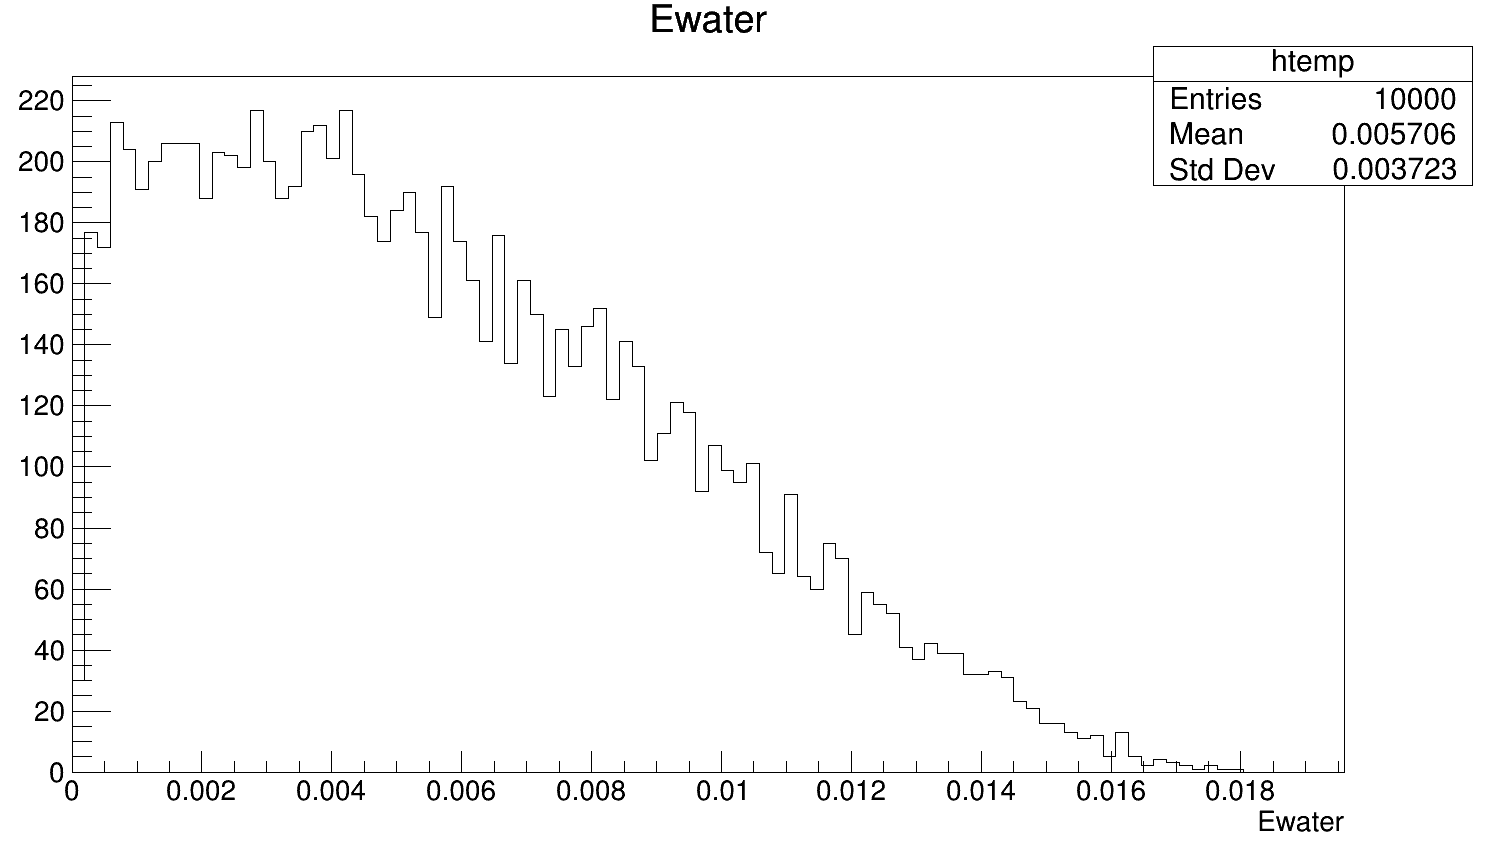
\includegraphics[scale=0.1]{deposicionenergiaagua.png} 
}
{
%\subfloat[Espectro de emisión]
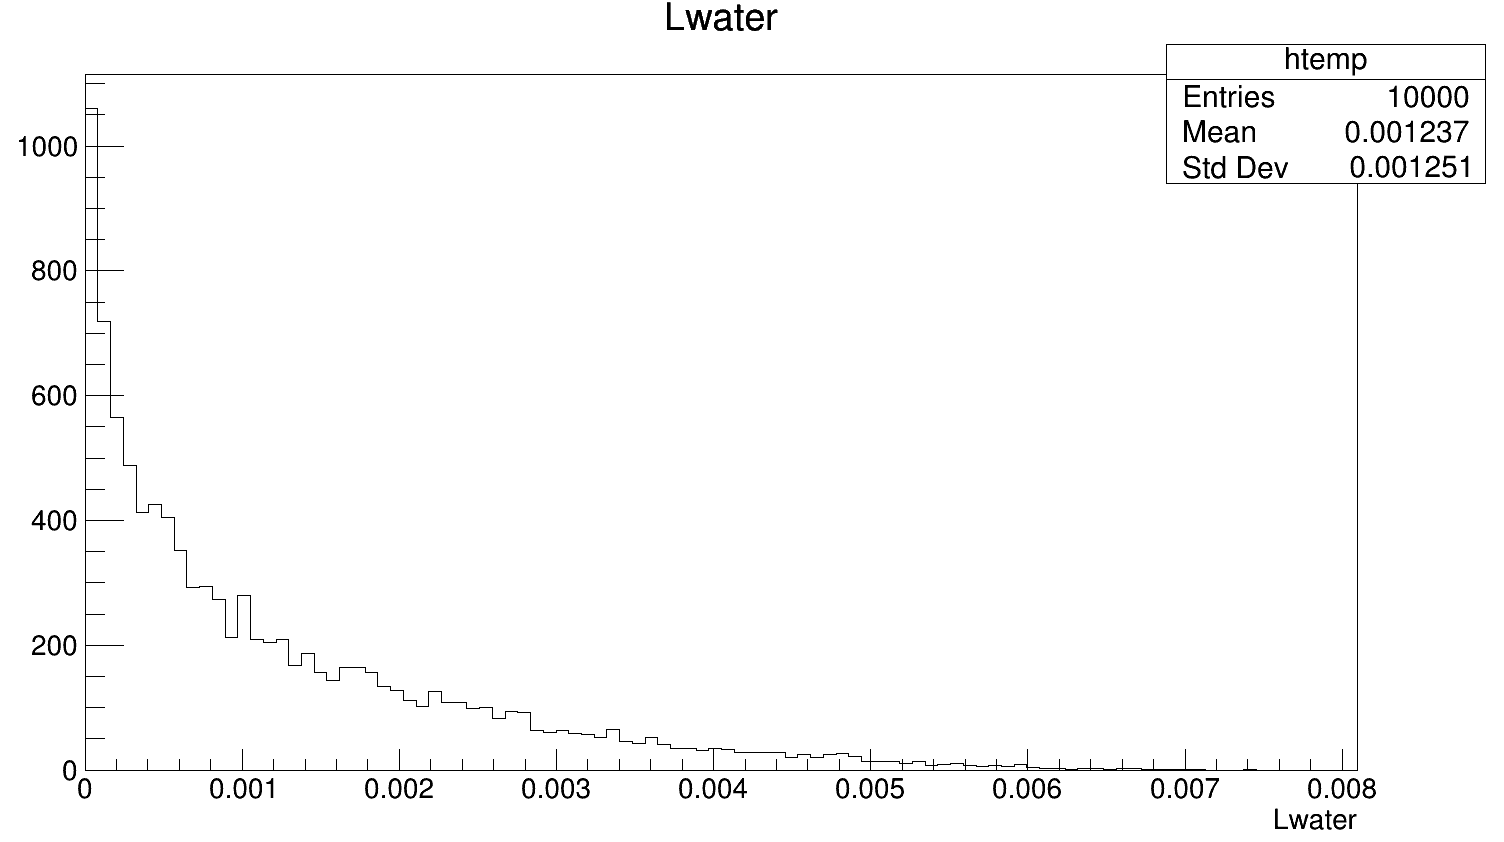
\includegraphics[scale=0.1]{longitudrecorridaagua.png} 
}
\caption{Histograma energético y espacial de los electrones absorbidos en al agua\label{deposicionagua}}
\end{figure}

\begin{figure}[htb]
\centering
{
%\subfloat[Espectro de emisión]
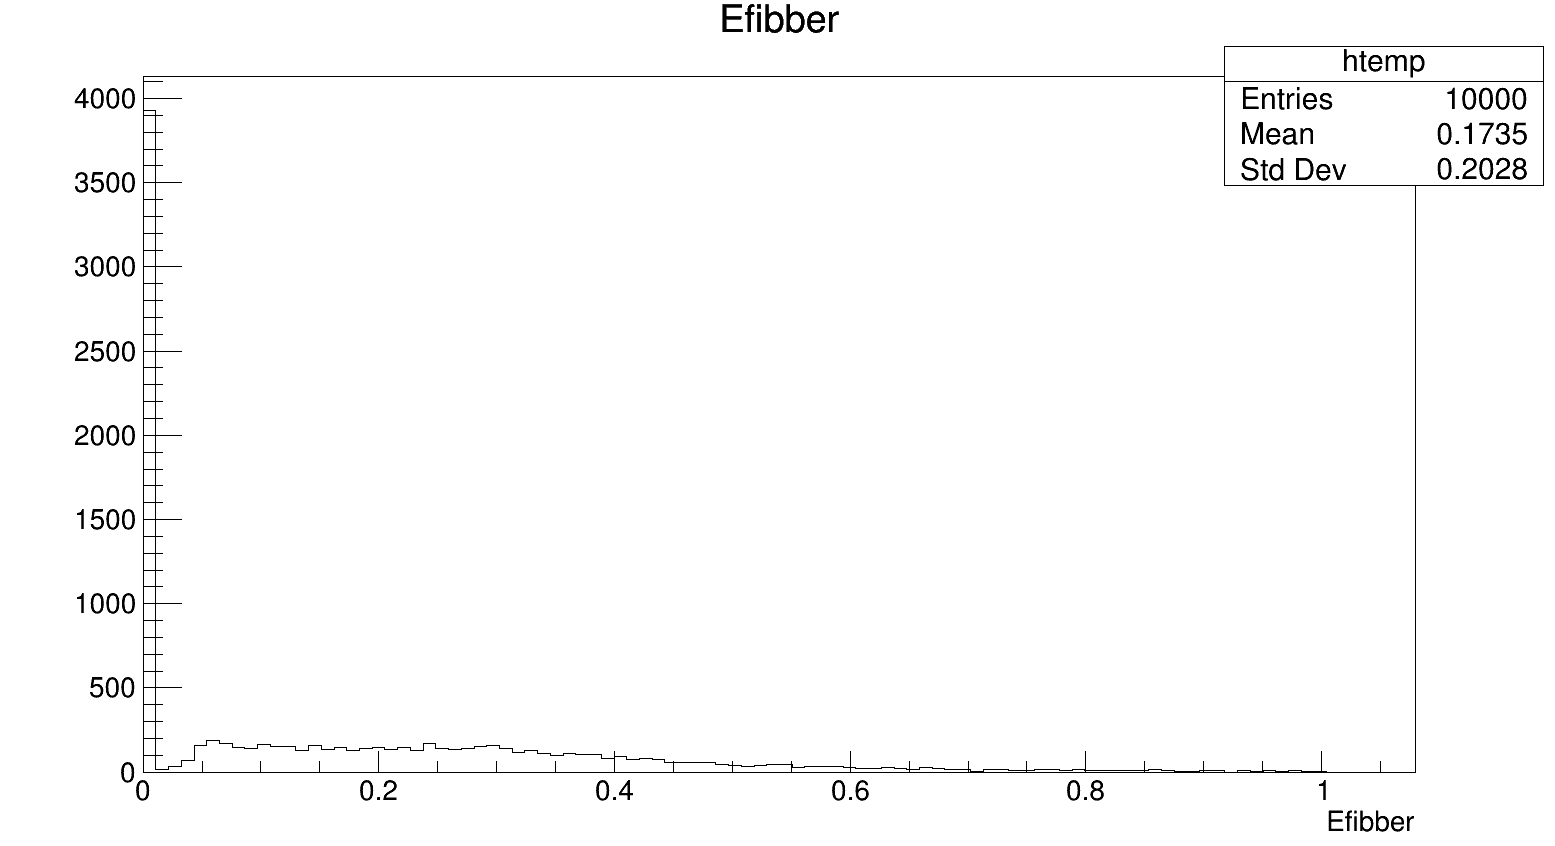
\includegraphics[scale=0.1]{energiadeposicionfibras.png} 
}
{
%\subfloat[Espectro de emisión]
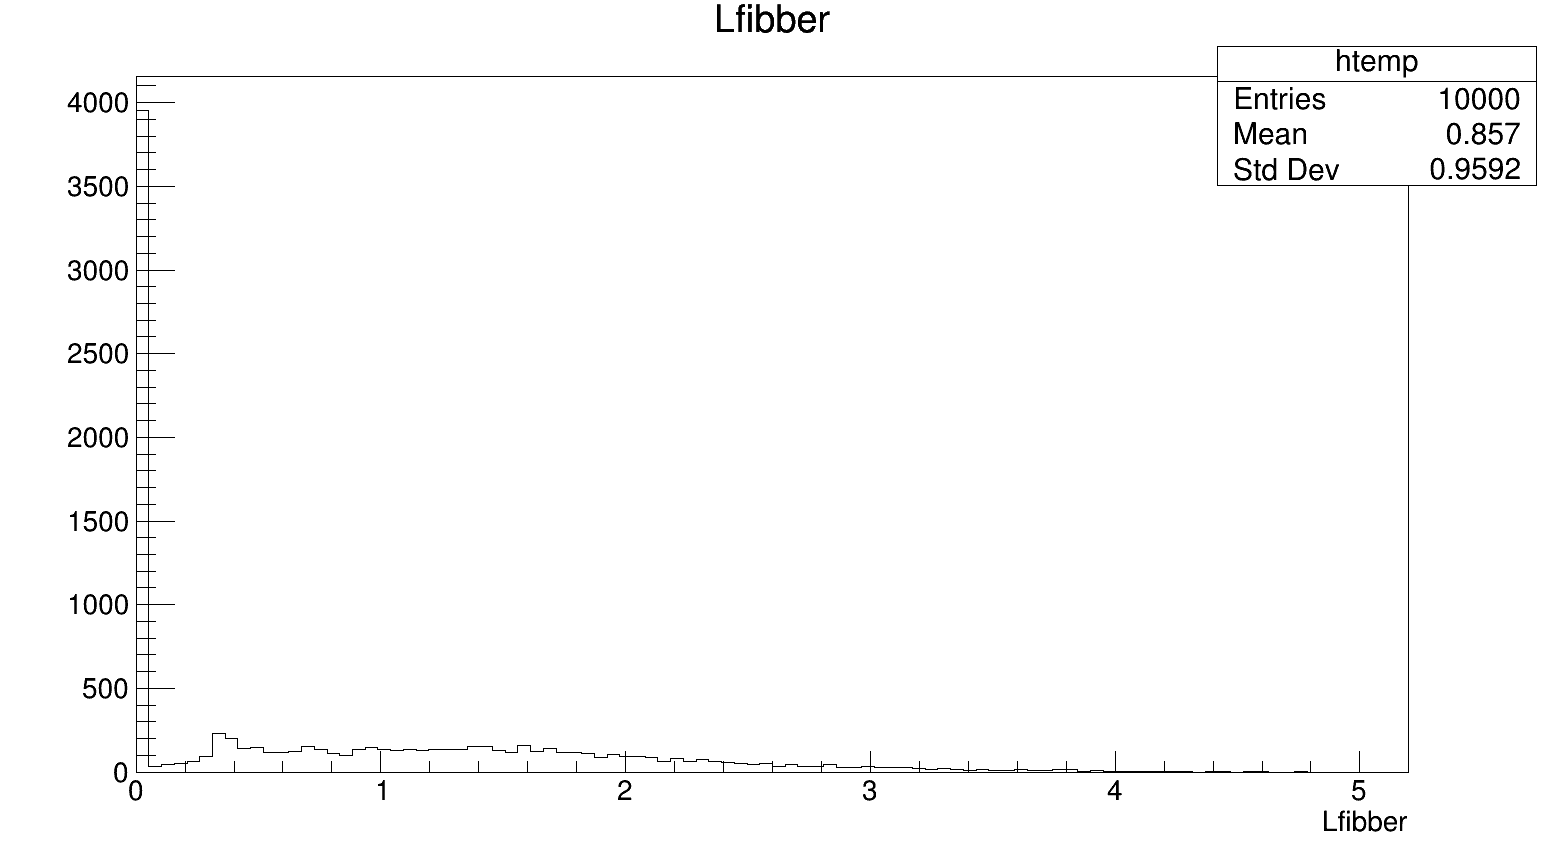
\includegraphics[scale=0.1]{longitudfibras.png} 
}
\caption{Histograma energético y espacial de los electrones absorbidos en las fibras\label{deposicionfibras}}
\end{figure}

En la figura 31 podemos observar que la energía depositada presenta un espectro típico de una desintegración $\beta$ y la longitud recorrida por los electrones presenta un decaimiento exponencial, función que, teóricamente, describe el fenómenos de atenuación, $N=N_0\exp{(-x/\lambda)}$. 

Podemos observar por tanto que el programa esta simulando correctamente la absorción de tritio en el agua. Algo similar ocurre en la imagen 32 pero en estos histogramas no puede apreciarse debido a limitaciones que presentaba el código desarrollado.

\item{} Finalmente se ha obtenido un histograma del número de fotones reemitidos en cada detección del tritio. Este se muestra en la imagen 33.

\begin{figure}[hbtp]
\centering
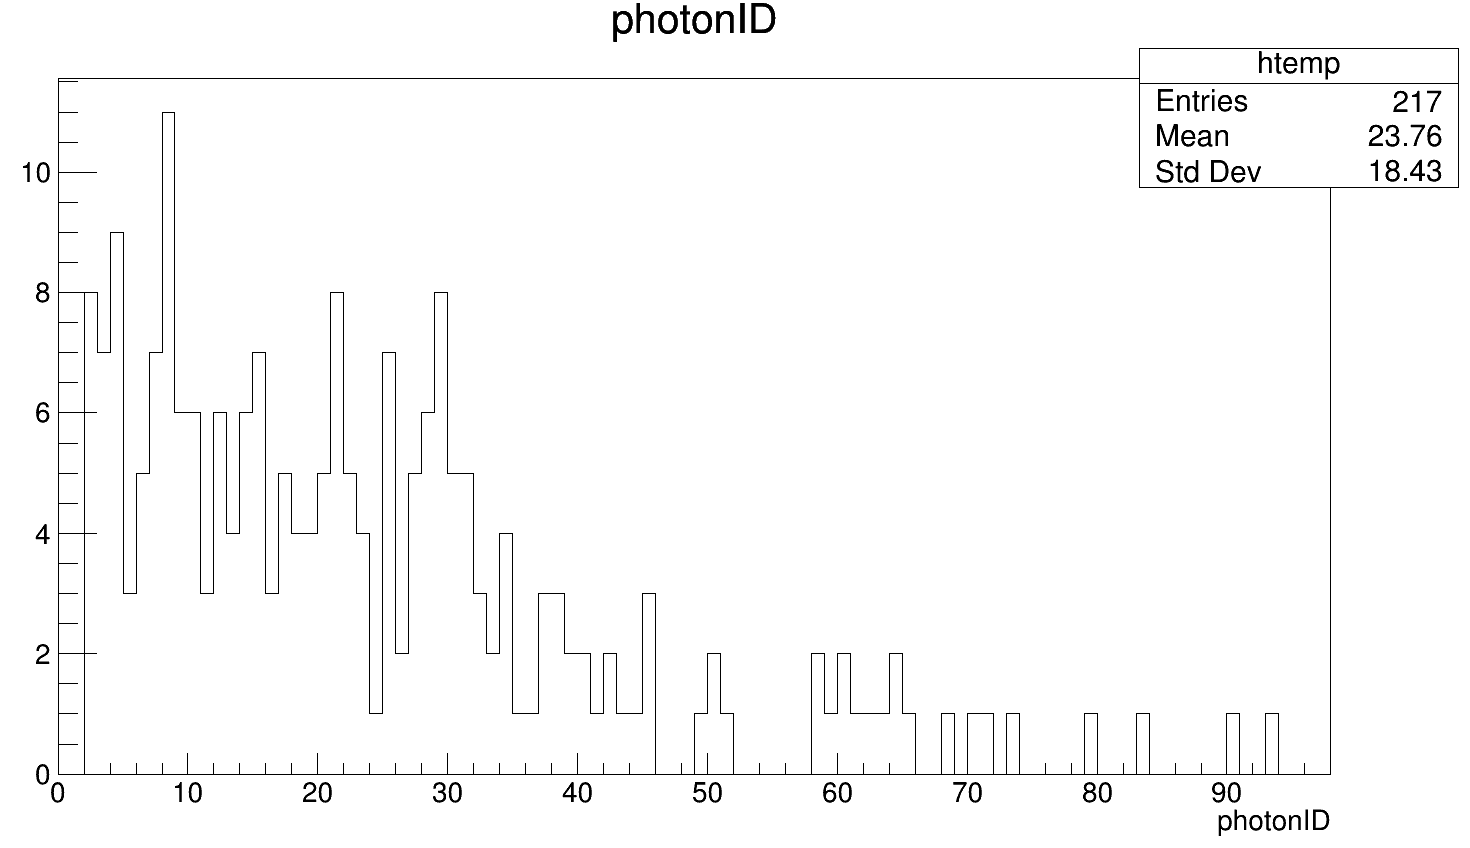
\includegraphics[scale=0.2]{reemisionfotones.png}
\caption{Histograma del número de fotones reemitidos en una detección \label{reemision}}
\end{figure}

Dado que existe una equivalencia entre la energía de la partícula detectada en la fibra y el número de fotones que esta reeemite deberíamos esperar un espectro similar a una desintegración $\beta$, fig. $\ref{Espectrotritio}$. Podemos observar que, efectivamente, se cumple.

Hay que tener en cuenta que solo han sido detectados y transformados en luz 217 eventos. Vemos por tanto que el espectro queda muy poco definido. De nuevo, para una mayor suavidad del espectro será necesario acceder al centro de cálculo del IFIC para disponer de de una mayor potencia de computación.
\end{enumerate}

Vemos por tanto que se ha realizado una simulación cuyo funcionamiento ha sido verificado. El siguiente paso sera desarrollar la parte del tratamiento posterior de la luz tanto a traves de las fibras como su detección en el contador de fotones. De esta forma podremos comprobar la importancia del guiado en las fibras centelleadoras.

\newpage
\section{Previsiones de futuro} \label{sec:ch04}
Como ya se ha mencionado duranto todo el trabajo, este dispositivo es un prototipo. La forma de proceder de \textit{Tritium}, y en general de un experimento, es realizar todas las medidas posibles sobre este y, cuando ya no podamos obtener más información, fabricar un nuevo prototipo que supere las limitaciones encontradas en el anterior. Nuevamente, realizar la misma labor sobre el siguiente prototipo. Se considerará que se ha llegado al diseño final cuando hayamos llegado al objetivo final del proyecto \textit{Tritium} (detectar actividades del orden de cientos de $\becquerel/L$) o ya no podamos aplicar mejoras para conseguir una optimización del sistema de detección y poder, de esta forma, detectar niveles de actividades más bajas.

Según se ha calculado realizado en la seccion $\ref{sec:Resultados}$ nuestro dispositivo presenta una actividad aproximada de $108,11~\mega\becquerel/L$. Podemos observar que todavía estamos lejos del límite actual ~\cite{Rat}, por lo que, según se ha explicado, el siguiente paso es pasar a diseñar una nueva versión del prototipo. 

Hay que tener en cuenta que aun podemos realizar una serie de medidas sobre el prototipo, tales como el cálculo de su eficiencia de fotodetección, los cuales nos permitirá determinar otras posibles mejoras que serán implementadas en el siguiente prototipo. Es importante obtener el máximo de información de cada prototipo para poder incluir una mayor optimización en la siguiente versión y, de esta forma, necesitar un menor número de prototipos para llegar al diseño final (abaratando de esta forma el proceso de I+D). 

A pesar de que todavía se realizarán más medidas sobre el prototipo final ya se han encontrado ciertas limitaciones de este prototipo que serán subsanadas  en la siguiente versión. Estas se citan a continuación:
\begin{enumerate}
\item{} En primer paso será la realización de medida con los SiPM con los que se realizó la calibración (Sec. $\ref{sec:SiPM}$) ya que recordemos que el prototipo utilizado hasta el momento únicamente ha utilizado PMT. El punto más importante de la sustitución de los PMTs por los SiPMs será la obtención de una mayor eficiencia del sistema, ya que los PMTs poseen una eficiencia bastante inferior, $30\%$, en comparación con los SiPMs, $50\%$.

Para poder depositar de forma segura los SiPM sobre el prototipo sera necesario el diseño de nuevas piezas de sujeción ya que las actuales (Fig. $\ref{tapones}$) estaban específicamente diseñadas para la sujeción de los PMT.

\item{} Hay que tener en cuenta que se utilizaron los SiPM modelo S13360-1375CS de hamamatsu (Sec. $\ref{sec:Equipo}$). Estos se utilizaron de forma provisional ya que son los que estaban disponibles en el laboratorio de reacciones nucleares y su espectro de PDE cumplía con los requisitios del proyecto (Fig. $\ref{Espectros}$). Además estos son de tipo CS, es decir, disponían de dos terminaciones para una conexión rápida y no permanente. 

Sin embargo, la propuesta final de tritium sería utilizar fotomultiplicadores modelo S13360-6075PE,  que presentan exactamente las mismas características que los anteriormente mencionados pero con un mayor tamaño, superficie total activa de 6x6 $mm^2$, y, por extensión, mayor número de pixels (6000). Este mayor número de pixels repercute en un mayor rango dinámico. Además estos SiPM son de tipo PE, es decir, presentan unas terminaciones que tiene que ir soldadas a la placa por lo que, para su utilización, se necesita disponer de la placa final que se utilizará en el prototipo. 

Dado que estos tienen que ir dispuestos sobre la tarjeta final del prototipo retrasaremos su utilización y, por el momento, realizaremos todas las pruebas sobre los SiPM actualmente utilizados ya que ambos presentan exactamente las mismas características en casi todos los aspectos.

\item{} En tercer lugar se pretende sustituir la tarjeta conversora (Sec. $\ref{sec:Tarjeta}$), tarjeta reciclada de un proyecto anterior, por una tarjeta especialmente diseñada para nuestro fin o un fin similar. Antes de empezar a diseñar esta tarjeta busquemos más necesidades que puede presentar nuestra tarjeta para poder ser implementadas todas en el siguiente prototipo.

Por un lado, uno de los pilares fundamentales del proyecto \textit{Tritium} será crear un proceso de automatización que compense las variaciones de la ganancia debidas a cambios en la temperatura con variación voluntarias de la ganancia debidas a cambios en el voltaje operaiconal (Sec. $\ref{sec:Compensacion}$).

Por otro lado, el diseño final del detector que pretende desarrollar el proyecto \textit{Tritium} presenta un grán número de bunch de fibras centelleadoras, a priori es desconocido y que habrá que calcular con ayuda de simulaciones, y, por extensión, necesitaremos un gran número de SiPM en las terminaciones de cada extremo de estos bunch. Debido a ello nos encontramos con la necesidad de desarrollar un proceso de automatización de la calibración de los SiPM.  

Por todo ello la tarjeta que será diseñada para el segundo prototipo deberá de ser capaz de reproducir estas labores de automatización. Para empezar con el diseño a pequeña escala de este proceso de automatización se utilizará una tarjeta que solo contiene cuatro posibles entradas (cada una de las cuales estará asociada a un SiPM). Además dispone de varios caminos para realizar esta automatización (por medio de relés o multiplexores) y dispone de la posibilidad de obtener la señal amplificado o no. Esta nos permitirá determinar cual de todos estos caminos ofrece menos cross talk entre señales y, por extensión, mejores resultados. La tarjeta utilizada se diseño en el IFIC para el proyecto NEXT-100 cuyo proyecto presenta unos requisitos muy similares a los nuestros~\cite{Marc}. Esta tarjeta puede verse en la figura 26 izquierda.

Habrá que familiarizarse con el programa LabView, programa elegido para desarrollar el código de automatización ya que cumple con todos los requisitos impuestos por el proyecto, disponemos de trabajos anteriores muy similares a nuestro proyecto realizados con este programa por compañeros del IFIC y, además, el IFIC posee licencia para su uso. También habrá que familiarizarse con el uso de algún tipo de micorcontrolador capaz de realizar esta labor de automatización. En concreto se utilizaran Arduinos ya que son rápidos, eficaces y económicos. El ardiuno utilizado, Arduino Mega, puede verse reflejado en la figura 26 derecha.

\begin{figure}[htb]
\centering
{
%\subfloat[Espectro de emisión]
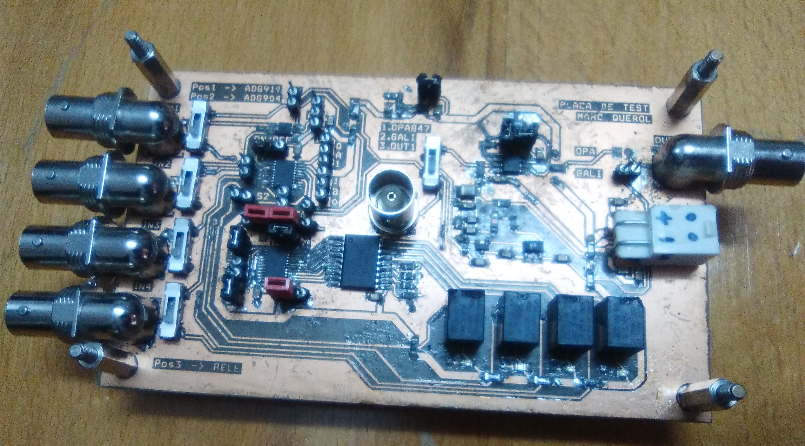
\includegraphics[scale=0.2]{Tarjeta1.png} 
}
{
%\subfloat[Espectro de emisión]
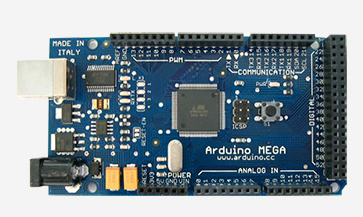
\includegraphics[scale=0.4]{Arduino.png} 
}
\caption{Tarjeta de automatización y Arduino Mega\label{arduino}}
\end{figure} 

Lo más importante de esta tarjeta es que por un lado realiza el proceso de automatización y, por otro, nos permite interaccionar con todas las partes importantes de nuestro experimento, tales como fuente de tensión de alimentación de distintos componentes del sistema, osciloscopios, etc, a partir de un programa llamado LabView.

Como ya se ha mencionado anteriormente esta tarjeta formará parte de un prototipo. El diseño final contendrá un número mucho mayor de bunch de fibras centelleadoras y, por extensión, necesitará un número mayor de SiPM para leer todas estas. Es en este punto cuando cobra una vital importancia el hecho de la automatización tanto en calibración de SiPM como en control de componentes ya que calibrar un número elevado de SiPM (en principio se han previsto 64 SiPM) es un trabajo que llevaría demasiado tiempo. Además, para poder controlar de forma efectiva un número tan elevado de SiPM es necesario un control automático. 

\item {} En cuarto lugar también habrá que proceder a contrucción de un clad para las fibras centelleadoras a partir del proceso de deposición de aluminio por evaporación en vacío el cula se realizará en el ICMOL, tema discutido en la sección $\ref{sec:Resultados}$.

\item {} En quinto lugar se ha visto que la medida obtenida del prototipo presenta una gran cantidad de ruido por lo que será un paso importante conseguir electrónica de bajo ruido en un futuro para poder seguir reduciendo la actividad del prototipo y que podamos distinguir esta señal del fondo.

\item {} En sexto lugar habrá que terminar las simulaciones incluyendo el posterior tratamiento de la luz tras su emisión en las fibras centelleadoras, tema que nos permitirá evaluar la importancia del guiado de luz en las fibras centelleadoras, tema discutido en la sección $\ref{sec:Resultados}$.

\item {} En séptimo lugar se desarrollará un segundo prototipo con una forma diferente ya que se vio que, aunque la forma de U sea la más segura para evitar posibles fugas, no es la más eficiente. En principio, los primeros diseños apuntan a un segundo prototipo rectilineo similar al de las simulaciones ya que, aparentemente, es el diseño en el que tendremos una menor pérdida por ángulo sólido.

\item {} En último lugar se pretende desarrollar un sistema de control de temperatura para disponer de este en el laboratorio de reacciones nucleares. Para ello se contruirá una caja de algún material términcamente asilante, por ejemplo poliespán, en el interior de la cual residirá nuestro foco frío y caliente. El foco frío consistirá en una resistencia térmica unida  a un ventilador de 12V y el foco frío consistirá en un aire acondicionado~\cite{Camara}.

\end{enumerate}

\newpage
\section{Conclusiones} \label{sec:conclusions}
El proyecto \textit{Tritium} ha realizado un primer paso construyendo un prototipo en forma de U cuyo interior, con una capacidad de $39~ml$, se ha rellenado con un una disolución de agua tritiada con una actividad de $108.11~\mega\becquerel/L$ (sec. $\ref{sec:Resultados}$).

Se ha conseguido obtener una señal del sistema a partir de la cual, mediante un tratamiento de datos \textit{off-line} que incluye la extracción del background, se ha obtenido una señal de actividad debida únicamente tritio (fig. $\ref{senaltritio}$). Este nos permite comprobar que el prototipo funciona correctamente ya que es capaz de discernir la presencia de tritio a partir de su contribución a la actividad total (background).

Sin embargo se ha visto que el prototipo presenta una eficiencia muy lejos de la idónea lo cual nos produce una numerosa pérdida de cuentas y, por extensión, una medida de la actividad que presenta el agua tritiada de su interior muy inferior en comparación con su valor teórico. 

Para comprobar hasta que punto es ineficiente nuestro prototipo se ha realizado una serie de estimaciones que nos han permitido determinar aproximadamente la actividad efectiva máxima que esperaríamos detectar con nuestro prototipo debido únicamente al agua tritiada, cuyo valor es $215.03~\becquerel$. En esta estimación se han tenido en cuenta eficiencias tanto de las fibras como de los fotomultiplicadores. 

Sin embargo, la actividad medida con nuestro prototipo es únicamente de $0.01\becquerel$, cuatro órdenes de magnitud por debajo del valor máximo. Podemos comprobar que se trata de una pérdida de cuentas realmente importante que produce un reordenamiento de prioridades en el proyecto ya que, de lo contrario, no podremos reducir la actividad del tritio en la muestra y seguir obteniendo señal. 

Ahora, la mayor prioridad y, por tanto, el tema sobre que tratarán las siguientes modificaciones en el prototipo será obtener una mayor eficiencia. Para ello el primer paso es determinar el punto en el que se ha producido esta pérdida de la señal. 

Se ha visto que un punto muy importante es el clad de la fibra, el cual permite una recolección eficiente de la luz. Debido a que las fibras utilizadas en el prototipo no presentan clad tenemos una gran pérdida de la señal en cada reflexión ($94\%$). Esto nos permite considerar que, aproximadamente, solo contirbuirán a la señal los fotones reemitidos por la fibra en la dirección del ángulo sólido cubierto por las caras finales de cada fibra, es decir, el ángulo sólido cubierto por las caras finales de bunch. 

A partir de una rápida estimación se ha visto que esto produce una considerable pérdida de cuentas llegando a factores del orden de $10^{-4}$ o $10^{-5}$ en distancias de apenas $2$ o $4~\cm$ respectivamente, valores que explicarían nuestra medida tan baja. Por tanto un primer paso en el siguiente prototipo será la utilización de fibras centelleadoras con clad. 

El incluir clad en las fibras centelleadoras será un proceso dificil y bastante laborioso ya que actualmente Saint-Gobain unicamente ofrece clads comerciales de aproximadamente $40~\mu m$, imposibilitando por completo su uso en este experimento ya que ningun electrón procedente de la desitnegración del tritio conseguiría cruzar el clad y aportar señal. Por tanto solo nos queda buscar algún método alternativo para obtener un clad. 

Se esta barajando la posibilidad de utilizar las instalaciones del ICMOL para realizar deposición de aluminio por evaporación en vacío, el cual nos permite llegar a grosores del orden de cientos de nanometros o menos. Sin embargo habrá que realizar un estudio sobre la aderencia ya que recordemos que las fibras se encontrarán en todo momento sumergidas en agua tritiada y necesitamos que el clad presente una adherencia mínima para permanecer en la fibra. También habrá que ver cual es el material que utilizaremos para conformar el clad. Lo ideal sería utilizar un materíal plastico sin embargo no se trata de una técnica estudiada para utilizar materiales no metálicos por lo que el hecho de hacerlo nos puede conducir a problemas.

También es ha visto la necesidad de cambiar la forma del prototipo ya que, de la forma actual, forma de U, la parte del bunch de fibras (aproximadamente el $33\%$) no contribuye a la señal ya que necesita un número excesivo de reflexiones para llegar al PMTs y, en cada una de estas existirá siempre una mayor o menor pérdida de la señal.

Por tanto, de todo también esto podemos ver que un punto decisivo será avanzar en las simulaciones para determinar el grosor y el material del clad, el diseño del prototipo, etc que optimicen la señal obtenida por el sistema. También nos permitirá estar preparados para superar de la mejor forma futuros problemas que nos encontraremos.

En último lugar también se han comentado futuros cambios que ya se estan estudiando pero cuya importancia es menor y podemos aplazar para un futuro tales como la automatización del sistema, utilización de electrónica de bajo ruido, etc.

\section{Agradecimientos} \label{sec:conclusions}
En primer lugar quería agradecer a mis dos tutores, Jose Díaz y Nadia Yahlali, el intentar transmitirme en todo momento el máximo de conocimientos posibles, iendo en muchas ocuasiones más allá de los conocimientos correspondientes a este trabajo. Por facilitarme cualquier tipo de herramienta o material que agilizase mi proceso de aprendizaje o mi trabajo. Agradecer en concreto que me haya facilitado las medidas de calibración de los PMTs utilizados en el prototipo además de ciertas macros de ROOT, desarrolladas por ellos mismos, que utilicé para aprender a usar ciertas funciones de ROOT importantes para desarrollar las macros que se utilizaron en este trabajo. También por informarme acerca de muchas de las herramientas de las que se dispone en el laboratorio y, en general, de las que dispone el IFIC, algunas de los cuales no eran necesarios para el desarrollo del TFM. Por utilizar gran parte de su tiempo en ayudarme a solucionar muchos de los problemas que me han ido surgiendo en el laboratorio y por sus consejos en temas relacionados con la burocracia. Finalmente agradecer el haberme incluirme en todo tipo de procesos referidos al proyecto \textit{Tritium}. 

En segundo lugar agradecer a los ingenieros electrónicos de laboratorio que, apesar de no disponer de poco tiempo libre, intentar ayudarme en cualquier duda que tuviese o intentar facilitarme material que necesitase.

Agradecer a los investigadores del IFIMED que nos prestasen su tiempo e instalaciones para desarrollar la calibración de los SiPM (ya que se necesitaba de un sistema de control de temperatura).

Agradecer a Teresa Cámara y a Rosa Carrasco por realizar la disolución radiactiva, el proceso de llenado de esta en el prototipo y por facilitarme cualquier tipo de material o ayuda que necesitase.

\section{Bibliografía} \label{sec:bibliographia}
%\section {Bibliografía}
\begin{thebibliography}{99}
\bibitem{300TBq} \textsc{A. Tarancón}, \textsc{H. Bagán}, \textsc{G. Rauret}, \textsc{J.F. García},
\textit{Comprative study of pre-treatment procedures for $ce{^{3}H}$ monitoring in water samples from environmental protection programs}

\bibitem{TesisTritio} \textsc{Zoltán Köllo},
\textit{Studies on a plastic scintillator detector for activity measurement of tritiated water}

\bibitem{limiteMB} \textsc{Masao Matsuyama}, \textsc{Kenichi Takatsuka}, \textsc{Masanori Hara}, 
\textit{Sensitivity of a specially designed calorimeter for absolute evaluation of tritium concentration in water}

\bibitem{Limitetiempo} \textsc{Yuji Hatano}, \textsc{Masanori Hara}, \textsc{Hiroko Ohuchi-Yoshida}, \textsc{Hirofumi Nakamura}, \textsc{Toshihiko Yamanishi},
\textit{Measurement of tritium concentration in water by imaging plate}

\bibitem{Limite}\textsc{N.P. Kherani},
\textit{An alternative approach to tritium-in-water monitoring}

\bibitem{gel} \textsc{M. Herrans}, \textsc{N. Alegría}, \textsc{R. Idoeta}, \textsc{F. Legarda},
\textit{Sampling tritiated water vapor from the atmosphere by an active system using silica gel}

\bibitem{Anillo} \textsc{C. Bray}, \textsc{A. Pailloux}, \textsc{S. Plumeri},
\textit{Tritiated water detection in the 2.17 $\mu M$ spectral region by cavity ring down spectroscopy}

\bibitem{Fiber-optic} \textsc{K.W. Jang}, \textsc{D.H. Cho}, \textsc{W.J. Yoo}, \textsc{J.K. Seo}, \textsc{J.Y. Heo}, \textsc{J.-Y. Park}, \textsc{B. Lee},
\textit{Fiber-optic radiation sensor for detection of tritium}

\bibitem{asignatura} \textsc{Mª Victoria Castillo Gimenez},
\textit{Instrumentación nuclear} 

\bibitem{datasheet} \textsc{Saint-Gobain Crystals},
\textit{Scintillating Optical FIbers}

\bibitem{anguloytiempo} \textsc{David Sáez-Rodríguez}, \textsc{Kristian Nielson}, \textsc{Ole Bang}, \textsc{David John Webb},
\textit{Simple room temperature method for polymer optical fibre cleaving}

\bibitem{dependencias} \textsc{S.H. Law}, \textsc{J.D. Harvey}, \textsc{R.J. Kruhlak}, \textsc{M. Song}, \textsc{E. Wu}, \textsc{G.W. Barton}, \textsc{M.A. vanEijkelenborg}, \textsc{M.C.J. Large}
\textit{Cleaving of microsctructured polymer optical fibres}

\bibitem{tesisfibras} \textsc{Joel S. Gearhard},
\textit{Investigation of BCF-12 plastic scintillating coherent fiber bundle timing properties}

\bibitem{manual} \textsc{Thorlabs},
\textit{Guide to connectorization and polishing optical fibers}

\bibitem{Santos} \textsc{Joaquín Santos Blasco},
\textit{UNITARY ANALYSIS OF THE SCALAR SECTOR OF THE STANDARD MODEL}

\bibitem{Santos} \textsc{Joaquín Santos Blasco},
\textit{UNITARY ANALYSIS OF THE SCALAR SECTOR OF THE STANDARD MODEL}

\bibitem{string} \textsc{J. Marsano},
\textit{String Thery in the LHC Era} Lecture 3: Why do we need the Higgs? 
%~\cite{Ivo}
\end{thebibliography}

\end{document}